\documentclass[letterpaper]{article}
\usepackage[top=1in, bottom=1.25in, inner=1.25in, outer=1.25in]{geometry}
\usepackage[style=authoryear-comp]{biblatex}
\addbibresource{bibliography.bib}
\usepackage{float}
\usepackage{amsmath}
\usepackage{tabularx}
\usepackage{siunitx}
\usepackage{graphicx}
\usepackage{tikz}
\usepackage{subcaption}
\usepackage{booktabs}

\title{Using Bayesian Regression to Quantify Sexual Dimorphism in Extinct Taxa}
\author{Eric Campbell}
\begin{document}
\maketitle

\newcommand{\species}[1]{\textit{#1}}
\newcommand{\tyran}{\species{Tyrannosaurus rex}{}}
\newcommand{\psit}{\species{Psittacosurus lujiatunensis}{}}
\newcommand{\maia}{\species{Maiasaura peeblesorum}{}}
\newcommand{\normal}[2]{\ensuremath{\mathcal{N}\left(#1, #2\right)}}

\section{Introduction}
Sexual dimorphism is the difference in size, colour, or presence of a feature between different sexes in a species. For instance, generally human males are larger than females, male mallard ducks are colourfully ornamented while females are drab, and male deer have antlers while females do not. Sexual dimorphism is very common in extant species, but detection of sexual dimorphism in extinct taxa, especially vertebrates, has been more challenging. Essentially, there are two difficulties in determining sexual dimorphism in extinct taxa: the `sexual' part and the `dimorphism' part. Determining the sex of the individual fossil, in the absence of rare features (such as medullary bone or bacula) is extremely challenging \parencite{saittaEffectSizeStatistical2020}. Similarly, determining the mass or size of a feature from a fossil (such as those of dinosaurs) can be difficult \parencite[p.~126]{brusatte2012}. When trying to determine the level of sexual dimorphism, these problems compound each other.

There are several analytical methods which are commonly used. However, each of these has their weaknesses. The use of $t$ tests (for differences in the mean) or Hartigans' dip test (for unimodality) can suffer from low statistical power \parencite{mallonRecognizingSexualDimorphism2017} and in the case of $t$ tests a further difficulty is the prolonged growth period of most dinosaurs \parencite{honeProtractedGrowthImpedes2017}. As a result, positive results for dimorphism in dinosaurs are rare.

However, a proposed method in \cite{saittaEffectSizeStatistical2020} attempts to sidestep these difficulties by explicitly constructing growth curves for the different sexes. Herein is proposed a modification to that method in which Bayesian regression is used to recover a distribution of possible growth curves for each sex and subsequently applied to calculate the level of dimorphism.

\section{Methods}
The modification to the method in \cite{saittaEffectSizeStatistical2020} is presented below.

\begin{table}[H]
    \centering
    \caption{Method Comparison}
    \begin{tabularx}{\textwidth}{XX}
        \toprule
        \multicolumn{1}{c}{\cite{saittaEffectSizeStatistical2020}} & \multicolumn{1}{c}{Modification} \\
        \midrule
        Gather data: age (or a correlate) and character of interest (e.g. length) & \\
        Fit growth curve to population as a whole & \\
        Predict sex by assigning all samples above the population curve to one sex and all below to the other. & \\
        Fit separate growth curves to each predicted sex & Create a posterior distribution for sex-specific parameters (Bayesian regression) \\
        Calculate maximum likelihood level of dimorphism & Calculate posterior distribution for dimorphism \\
        \bottomrule
    \end{tabularx}
\end{table}

In both methods, the amount of dimorphism is calculated as the difference in the asymptotes of the growth curves.

\subsection{Method Validation}

Validating the method began with a simulated population of American alligators (\species{Alligator mississippiensis}). The original von Bertalanffy growth curves were determined in \cite{wilkinsonGrowthRatesAmerican1997} and a simplified model using a constant standard deviation (rather than sex-specific standard deviation of the form $\alpha \log(\text{mean mass at age}) + \beta$) was used to generate different samples. The final model was

\begin{align*}
\text{Length}_{ m / f } &\sim \mathcal{N}\left(\mu_{ m / f }, \sigma\right) \\
\mu_m &= 3.79 * \left(1 - 0.94e^{-0.0695 \ast \text{age}}\right) \\
\mu_f &= 2.78 * \left(1 - 0.91e^{-0.0926 \ast \text{age}}\right) \\
\sigma &= 0.25
\end{align*}

For the von Bertalanffy equation
$$
\text{Length} = L(1 - Ae^{-K \ast \text{age}})
$$

the parameter $L$ is the asymptotic length, and so the actual level of sexual dimorphism is $\SI{3.79}{\m} - \SI{2.78}{\m} = \SI{1.01}{\m}$.

\begin{figure}
	\centering
	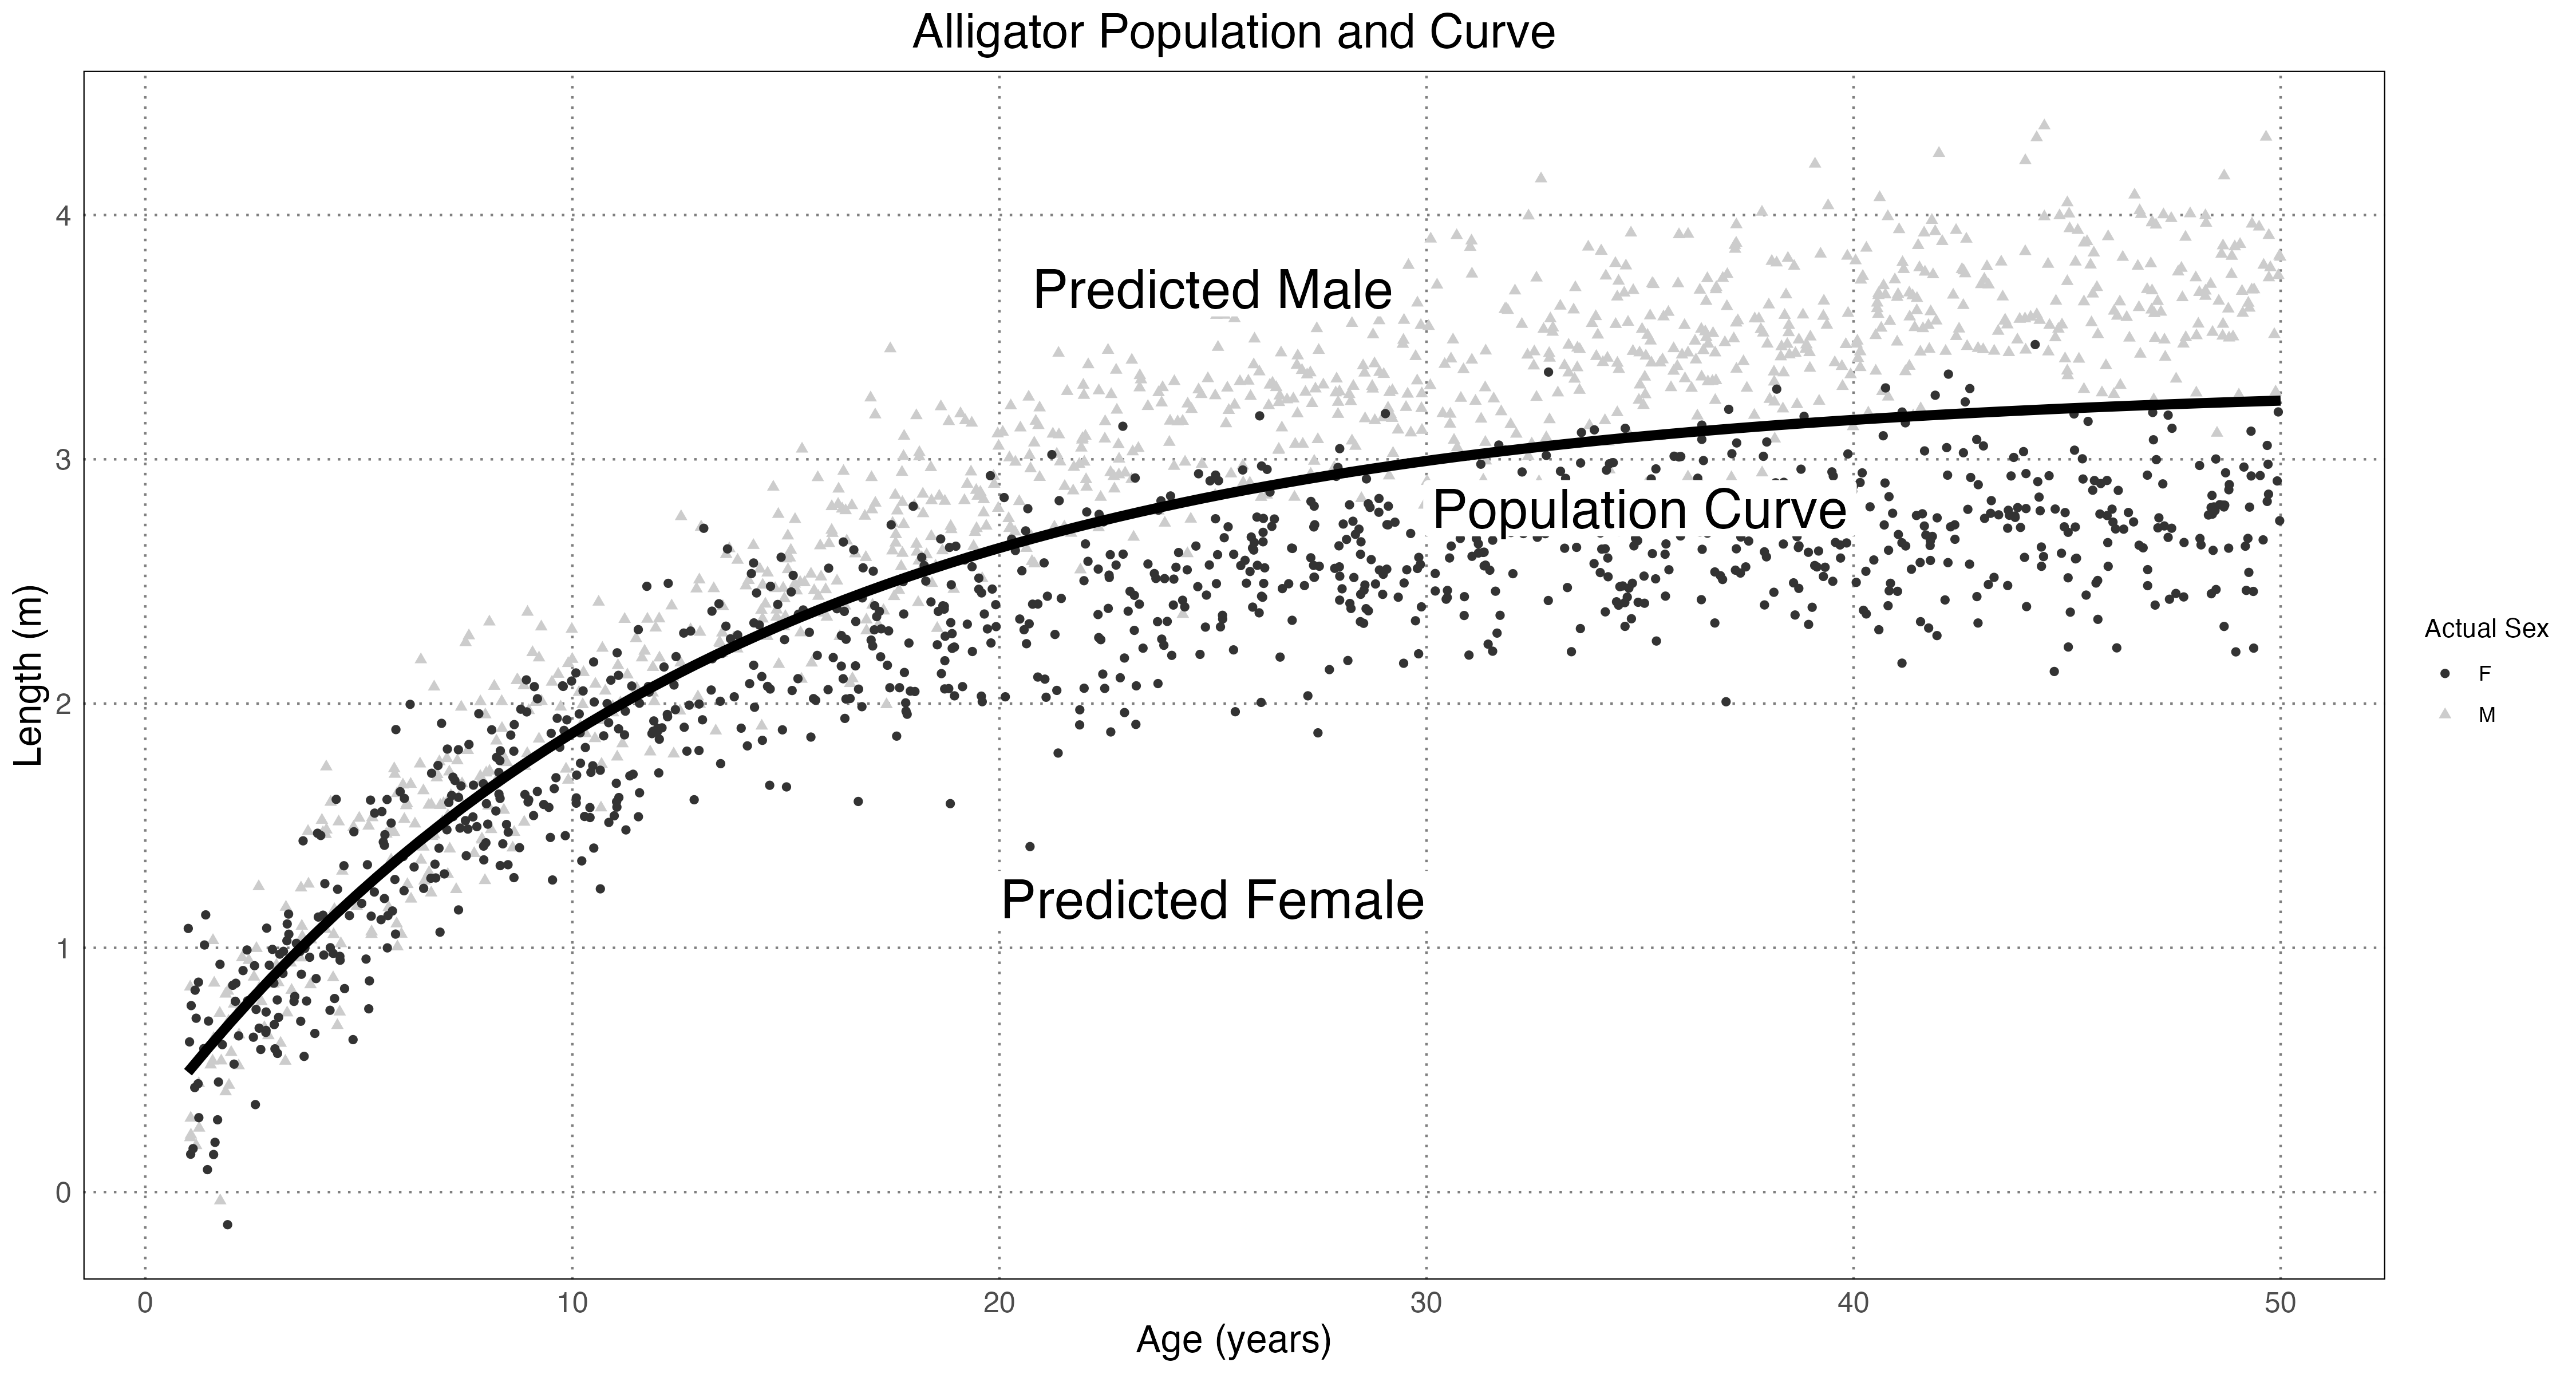
\includegraphics[width = \textwidth]{images/alligatorMethod.png}
	\caption{Simulated Alligator Populations \& Method}
	\label{fig:alligatorSim}
\end{figure}

 A Bayesian model with wide priors centred around the population-level curve values was used to recover the values \parencite{rCore, rstan}.

\begin{align*}
\text{Length}_{m/f,i} &\sim \normal{\mu_{m/f, i}}{\sigma} \\
\mu_{m/f, i} &= \text{von Betlananffy}(\text{age}_i, L_{ m/f }, A_{ m/f }, K_{ m/f }) \\
L_{ m/f } &\sim \normal{\text{population L}}{0.5} \\
A_{ m/f } &\sim \normal{\text{population A}}{0.025} \\
K_{ m/f } &\sim \normal{\text{population K}}{0.05} \\
\sigma &= 0.25 \\
\end{align*}

Since the priors used for the male and female parameters are identical (and initially have means equal to the population-level parameters), the results are slightly biased toward a finding of minimal or no sexual dimorphism.

Both when using only single sex (female) or when including both, the model was able to recover all of the population parameters with a high degree of accuracy (in all cases within the 95\% credible interval for the posterior of each parameter).

The sample size also affects the ability of the method to recover the true values. The model was run with several different sample sizes and the posterior distribution for the level of dimorphism $L_m - L_f$ is shown below.

\begin{figure}[H]
	\centering
	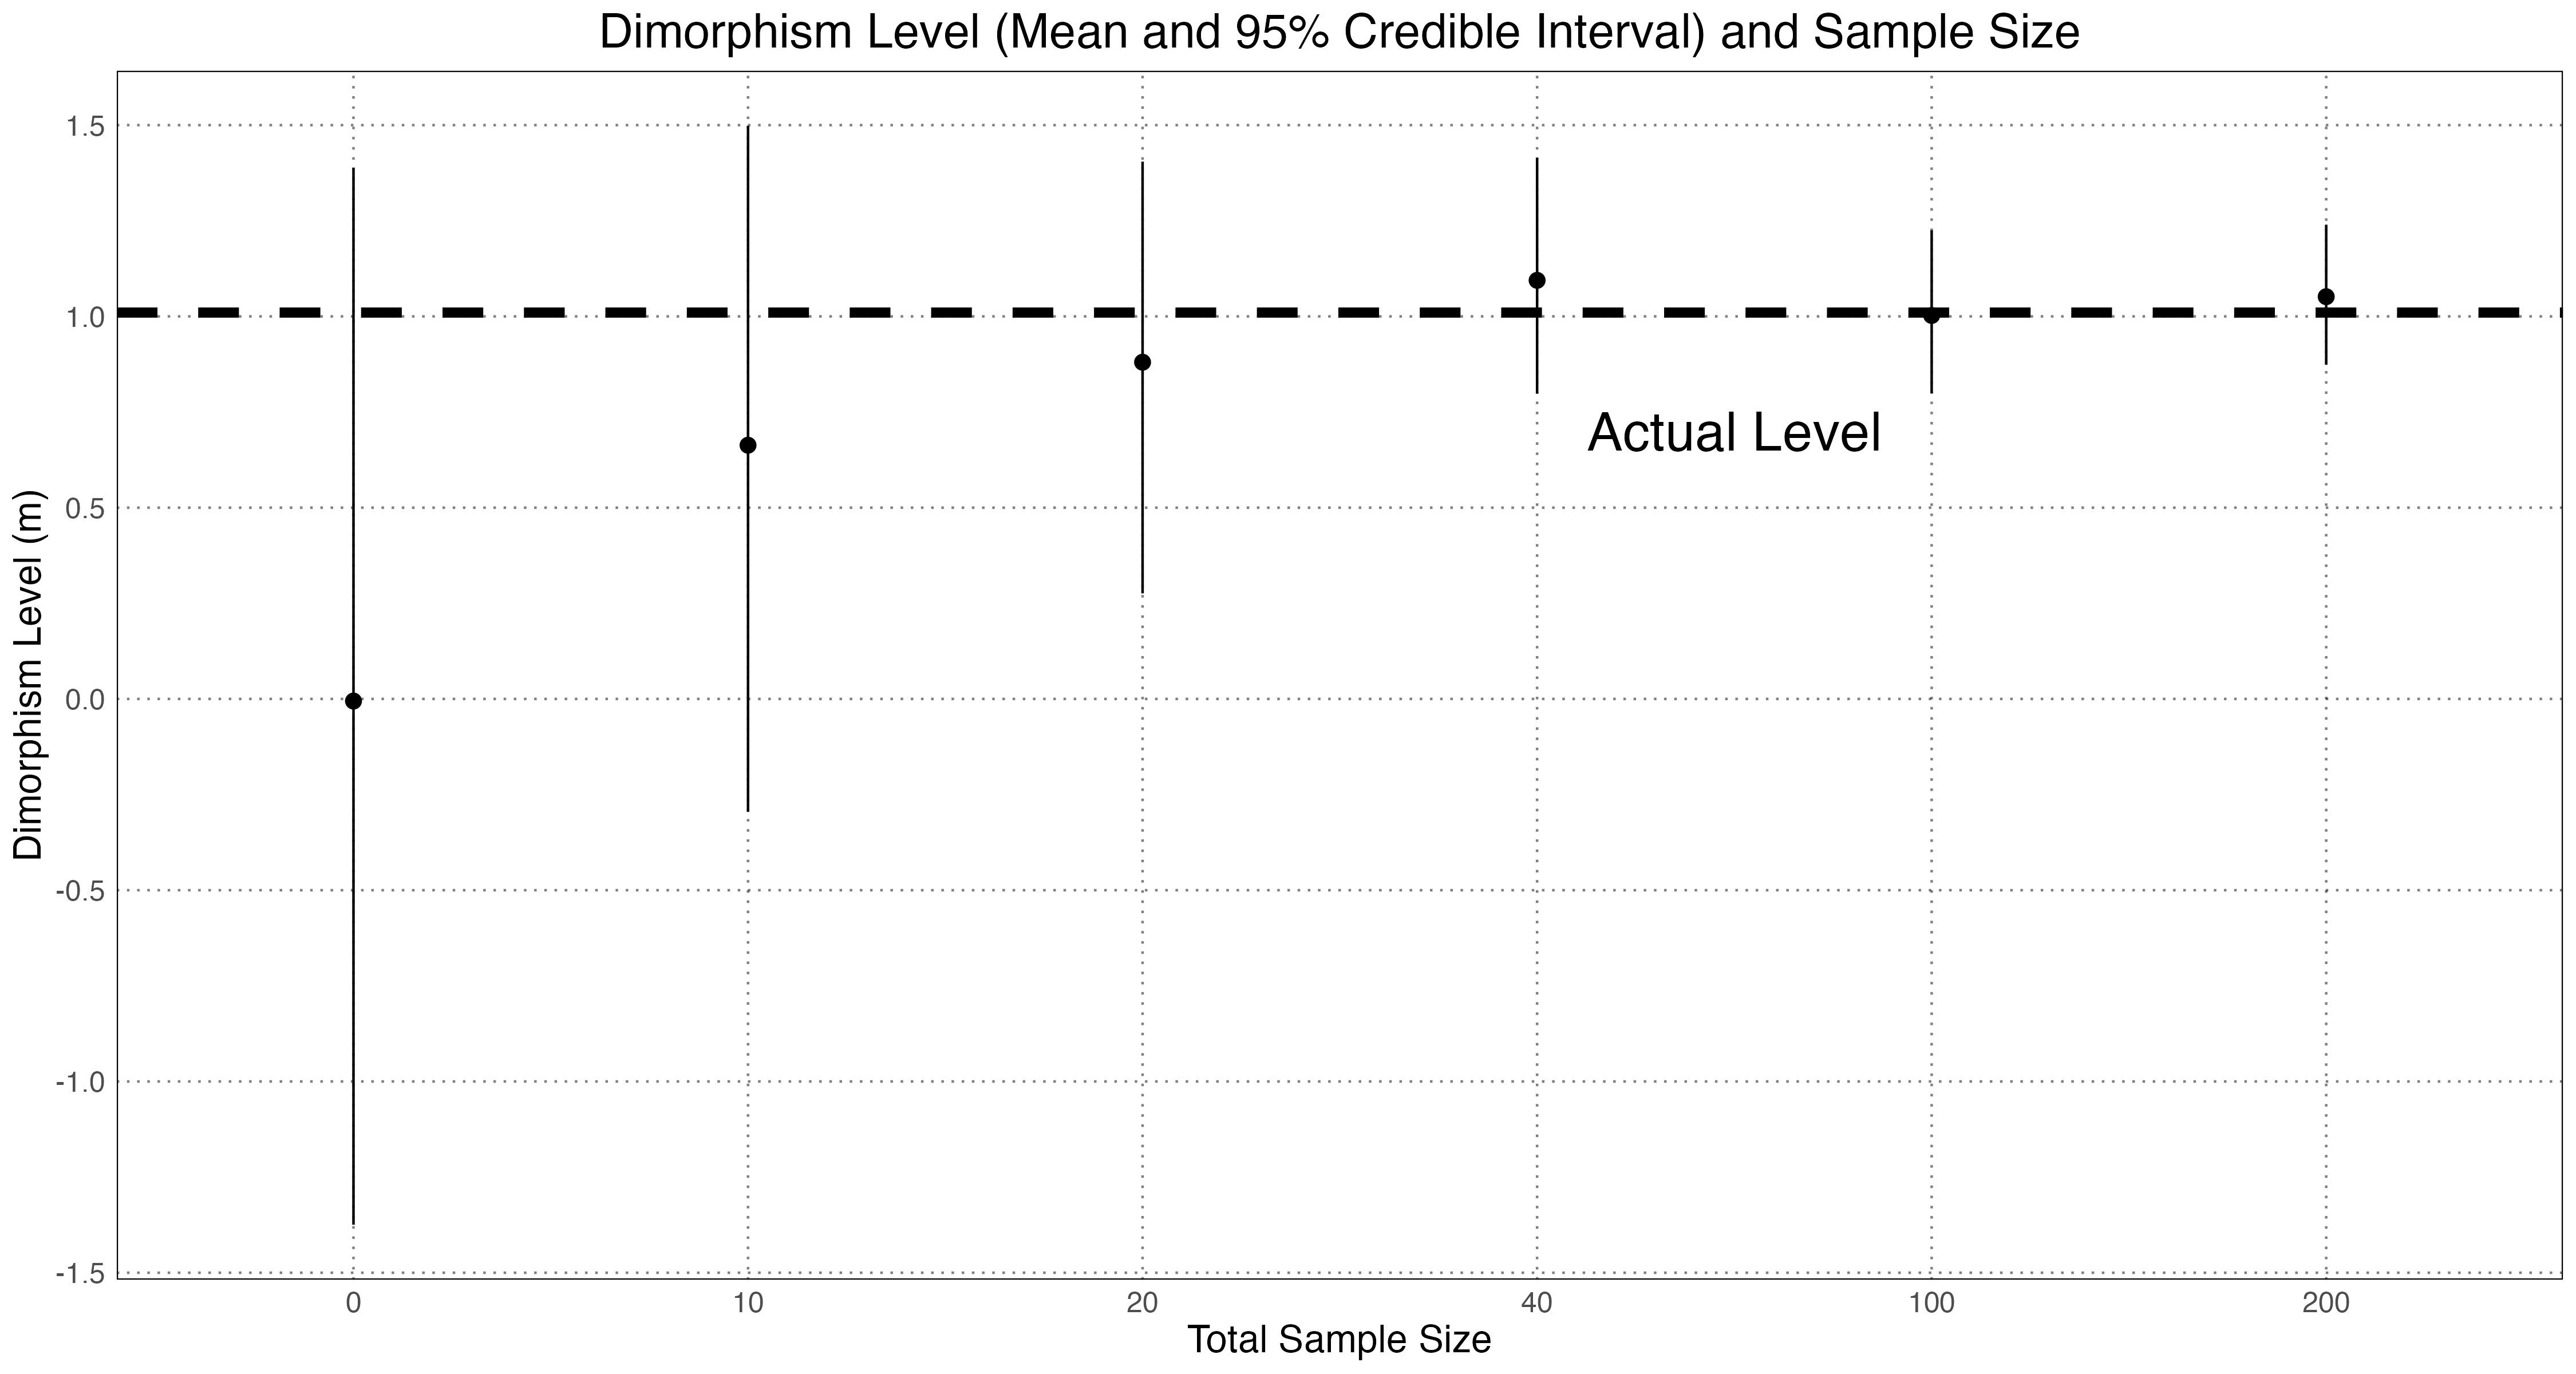
\includegraphics[width = \textwidth]{images/alligatorSampleSize.png}
	\caption{How different sample sizes affect the estimation of the level of dimorphism}
	\label{fig:alligatorSampleSize}
\end{figure}

This method reliably generates mean levels which are close to the true value and the 95\% credible intervals overlap it as well. The general pattern of approaching the value from below is due to the influence of the prior (centred at zero); as the sample size becomes larger they drag the posterior toward the correct value.

We can also ask about how the magnitude of dimorphism affects our ability to detect it. For this, the female parameters were kept at their original value and simulated male populations were created with an effect size $E$ representing the scaled difference between the actual male and female parameters. An effect size of $E = 0$ means that the male and female populations are identical, $E = 1$ is the natural level of dimorphism, and $E = 2$ is twice the natural level of dimorphism. The model was then run and the error in the level of dimorphism was calculated.

\begin{figure}[H]
	\centering
	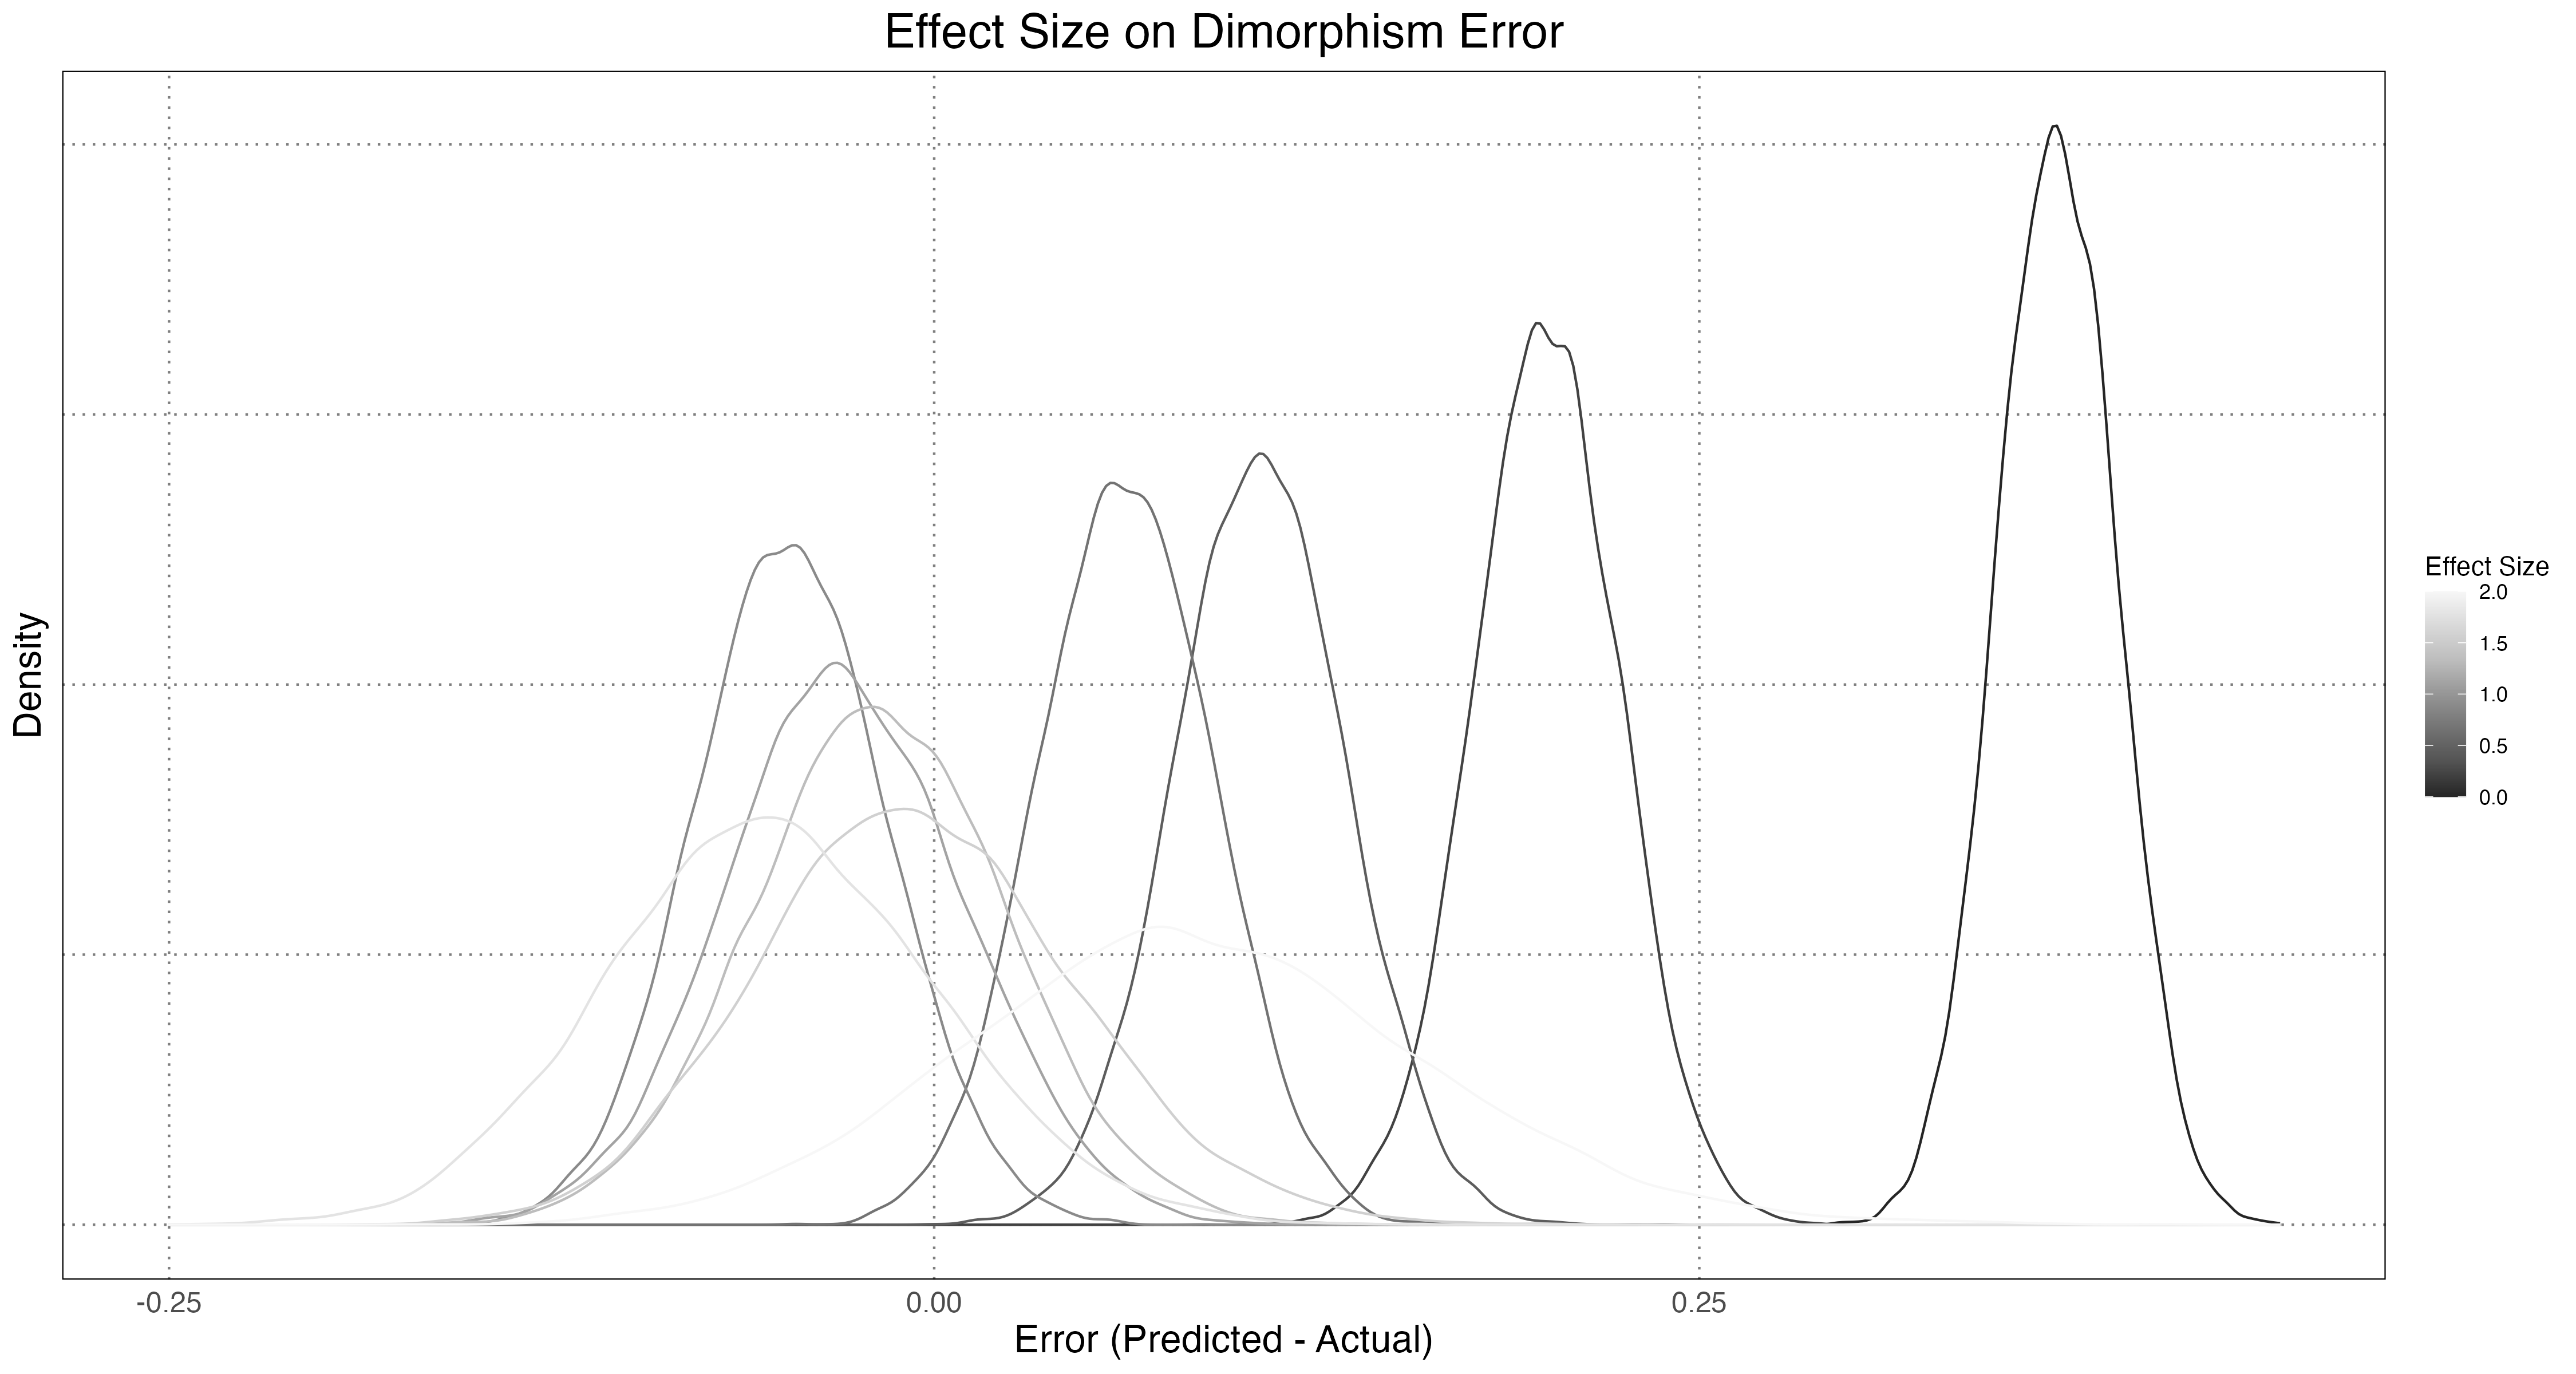
\includegraphics[width = \textwidth]{images/alligatorEffectSize.png}
	\caption{Effect of sample size on estimated dimorphism level}
	\label{fig:alligatorEffectSizes}
\end{figure}

There is a tendency to overestimate dimorphism when it is small, but converges to the correct value once it reaches a large enough size. Note that a significant contributor to the error in dimorphism estimation is the inaccuracy of our naive sex predictor. By plotting the accuracy of the dimorphism estimation against the computed accuracy in sex prediction, we can see a clear relationship.

\begin{figure}[H]
	\centering
	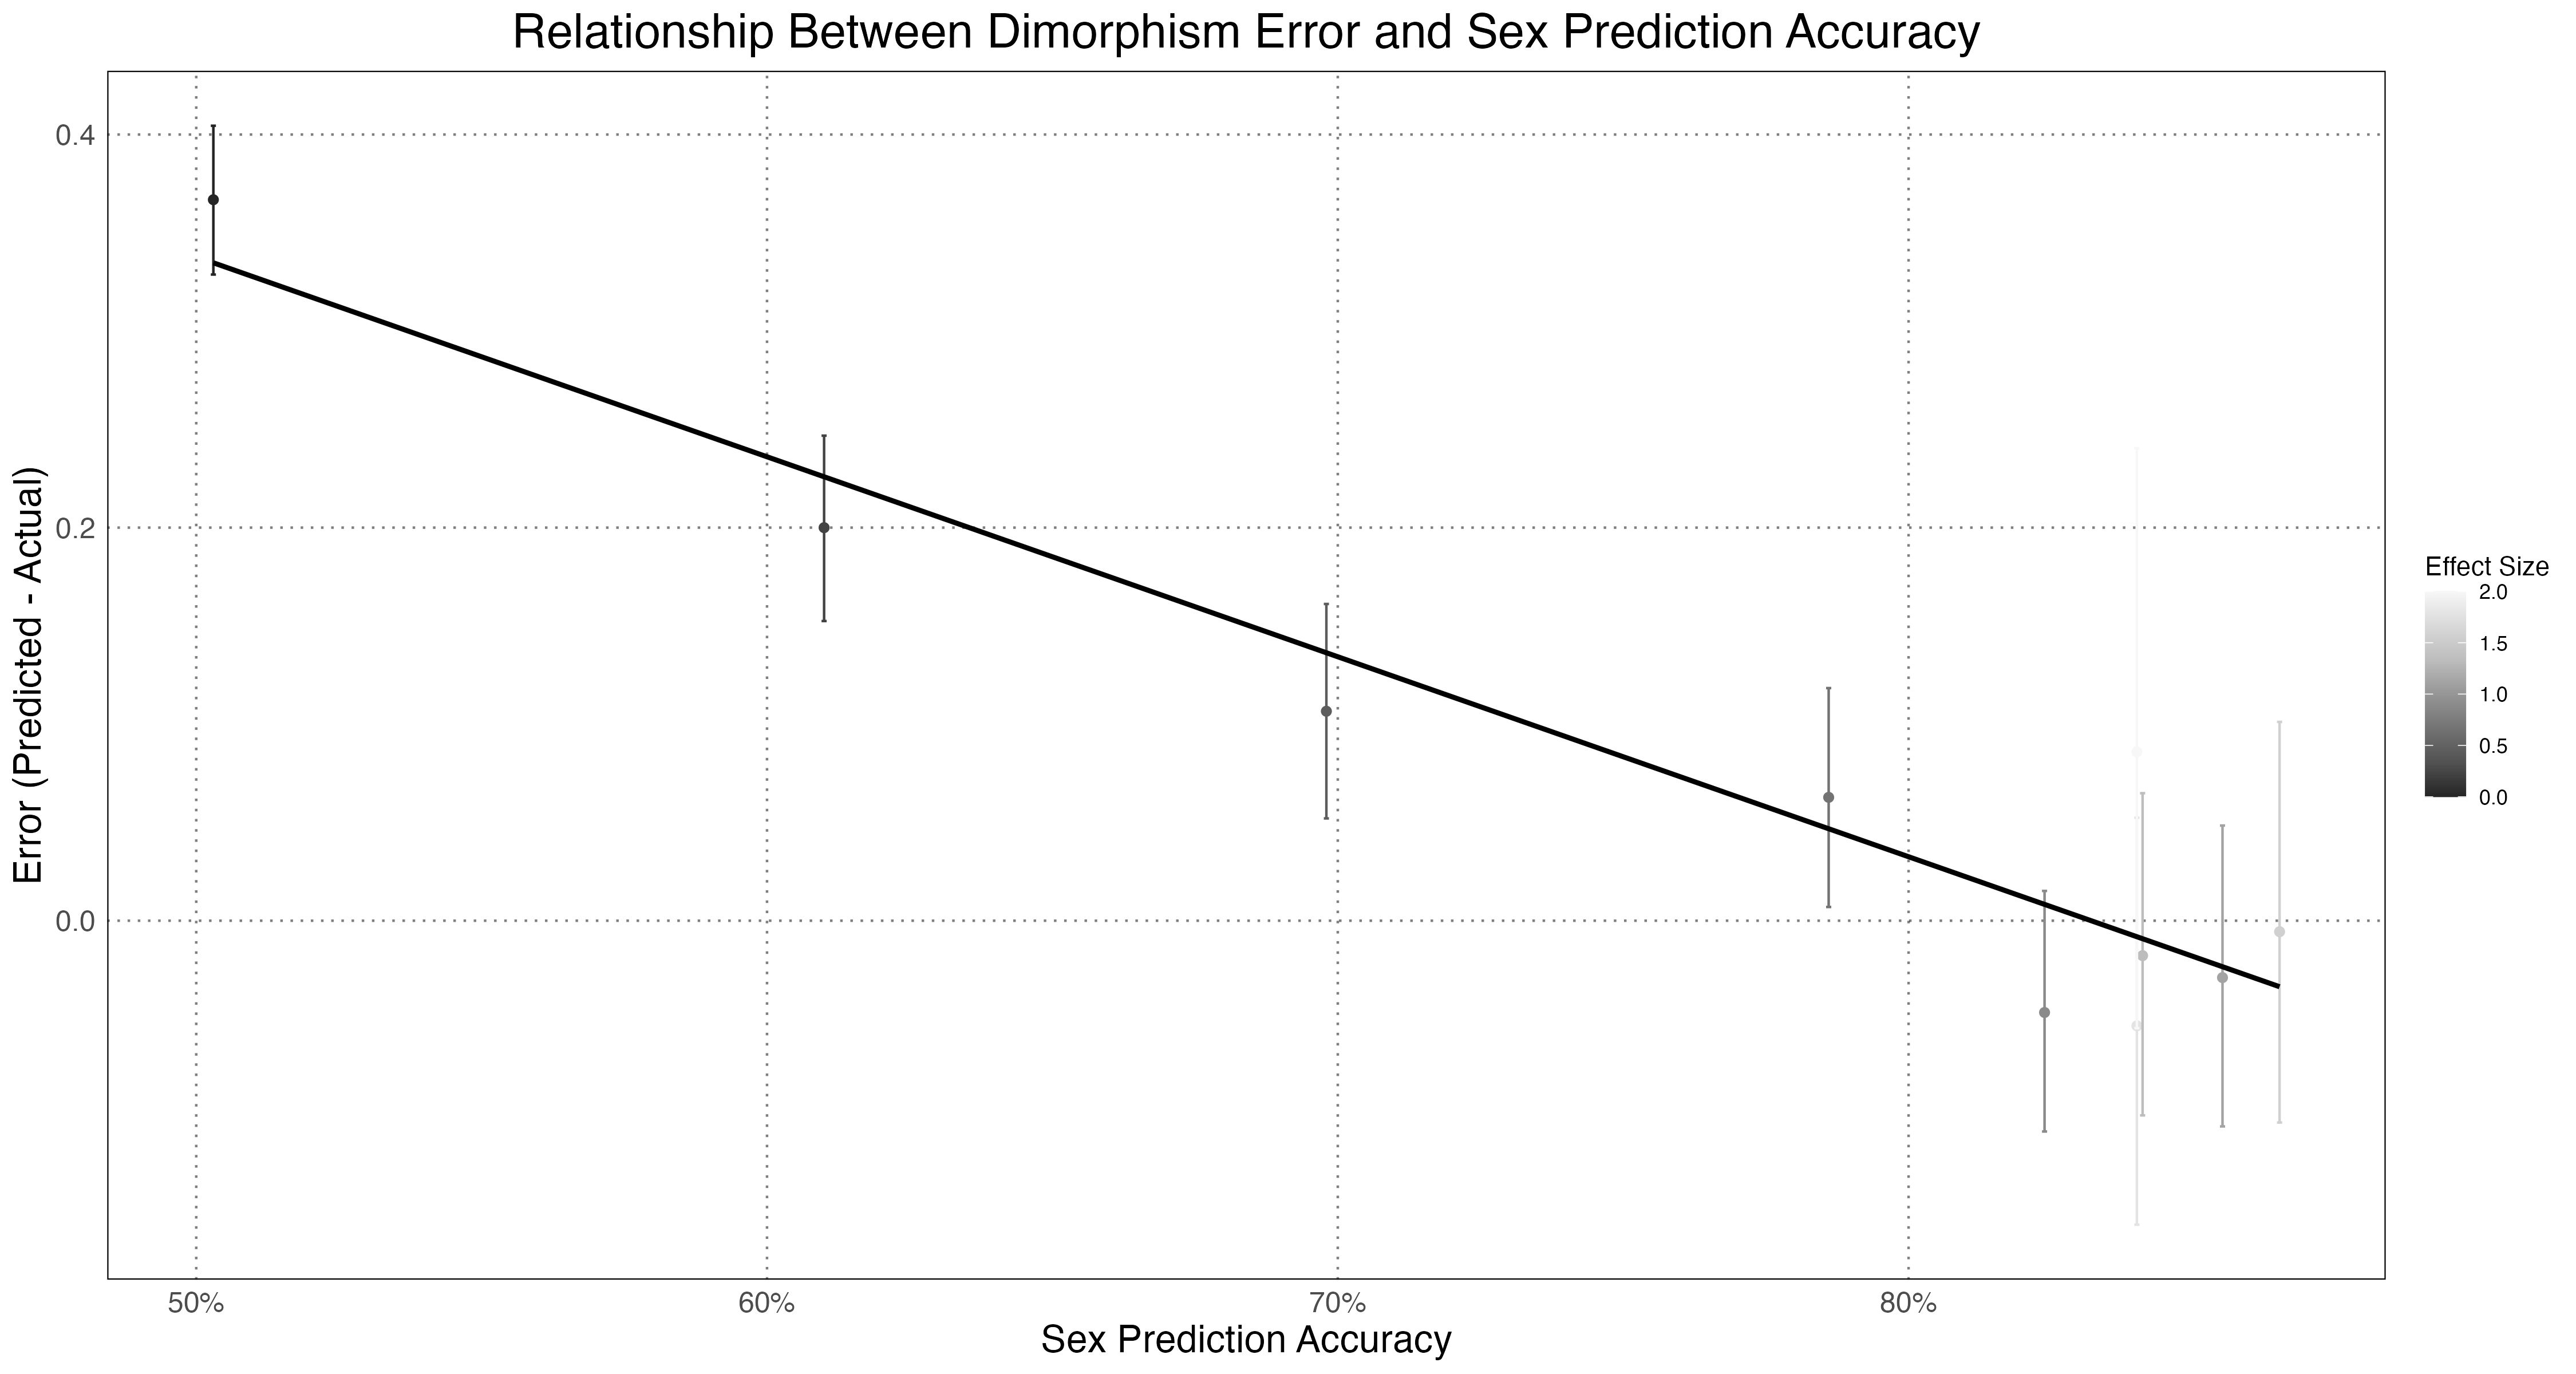
\includegraphics[width = \textwidth]{images/alligatorSexPredictionAccuracyDimorphismError.png}
	\caption{Relationship between the error in dimorphism estimation and the accuracy of sex prediction}
	\label{fig:alligatorSexPredictionError}
\end{figure}

Overall, the results of the simulation show that this method is reliable, with caveats that at low sample sizes or levels or dimorphism we need to be especially skeptical of the results.


\section{Results}

Once the method had been validated, the same method was used to calculate the posterior distribution for sexual dimorphism for three species of dinosaur: \maia{}, \psit{}, and \tyran{}. The data used were compiled in \cite{saittaEffectSizeStatistical2020} and were originally from \cite{woodwardMaiasauraModelOrganism2015} (\maia), \cite{ericksonFlawedAnalysisResponse2015}  (\psit), and \cite{ericksonGigantismComparativeLifehistory2004}, \cite{hornerAgeGrowthDynamics2004}, and \cite{leeSexualMaturityGrowing2008} (\tyran).

In each case, a logistic growth curve for mass against age with a constant standard deviation was used.

$$
\text{logistic}(\text{age}, L, q, k) = \frac{L}{1 + e^{q+k \ast \text{age}}}
$$

Since $L$ is the asymptotic mass, the level of dimorphism is $L_l - L_s$, where here $l$ represents the larger sex and $s$ represents the smaller one. For each species, priors were chosen again centred around the population level parameters and with a wide enough standard deviation to cover all of the existing data.

For each species, the prior 95\% quantiles for randomly generated populations, along with the actual data, are displayed, along with a selection of posterior growth curves.

\begin{figure}[H]
  \centering
  \begin{minipage}[b]{0.45\textwidth}
    \centering
    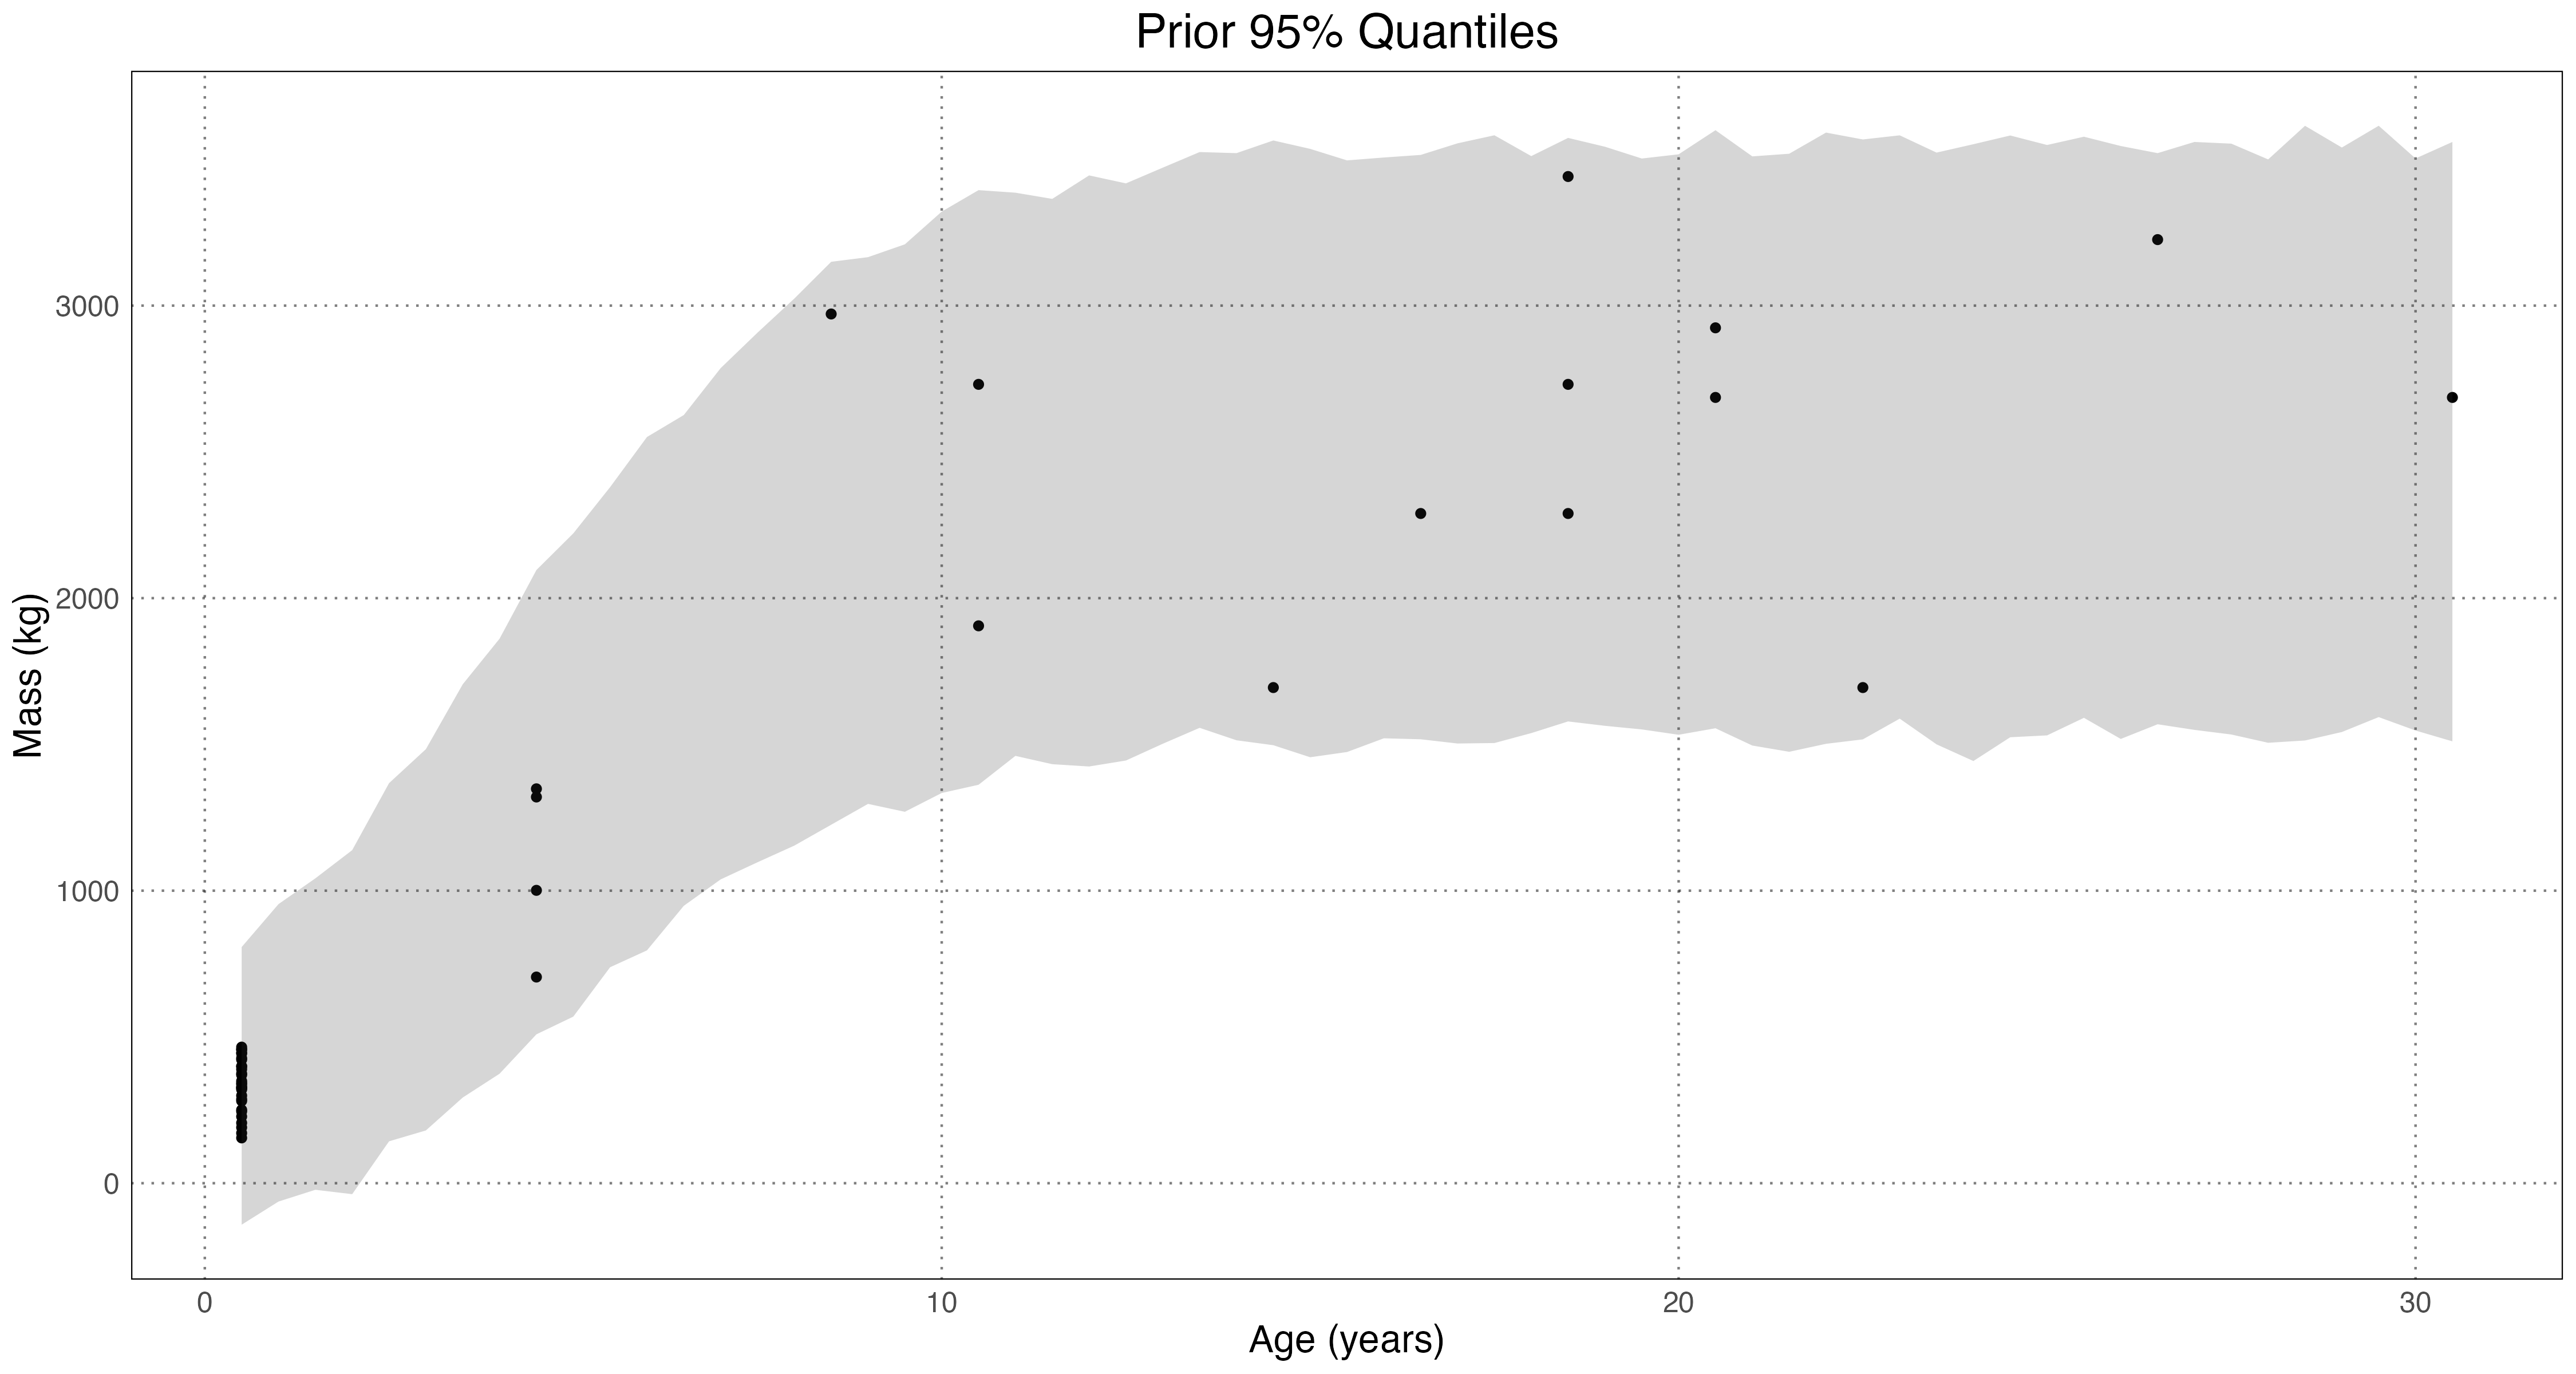
\includegraphics[width=\textwidth]{images/maiasauraPrior.png}
  \end{minipage}
  \begin{minipage}[b]{0.45\textwidth}
    \centering
    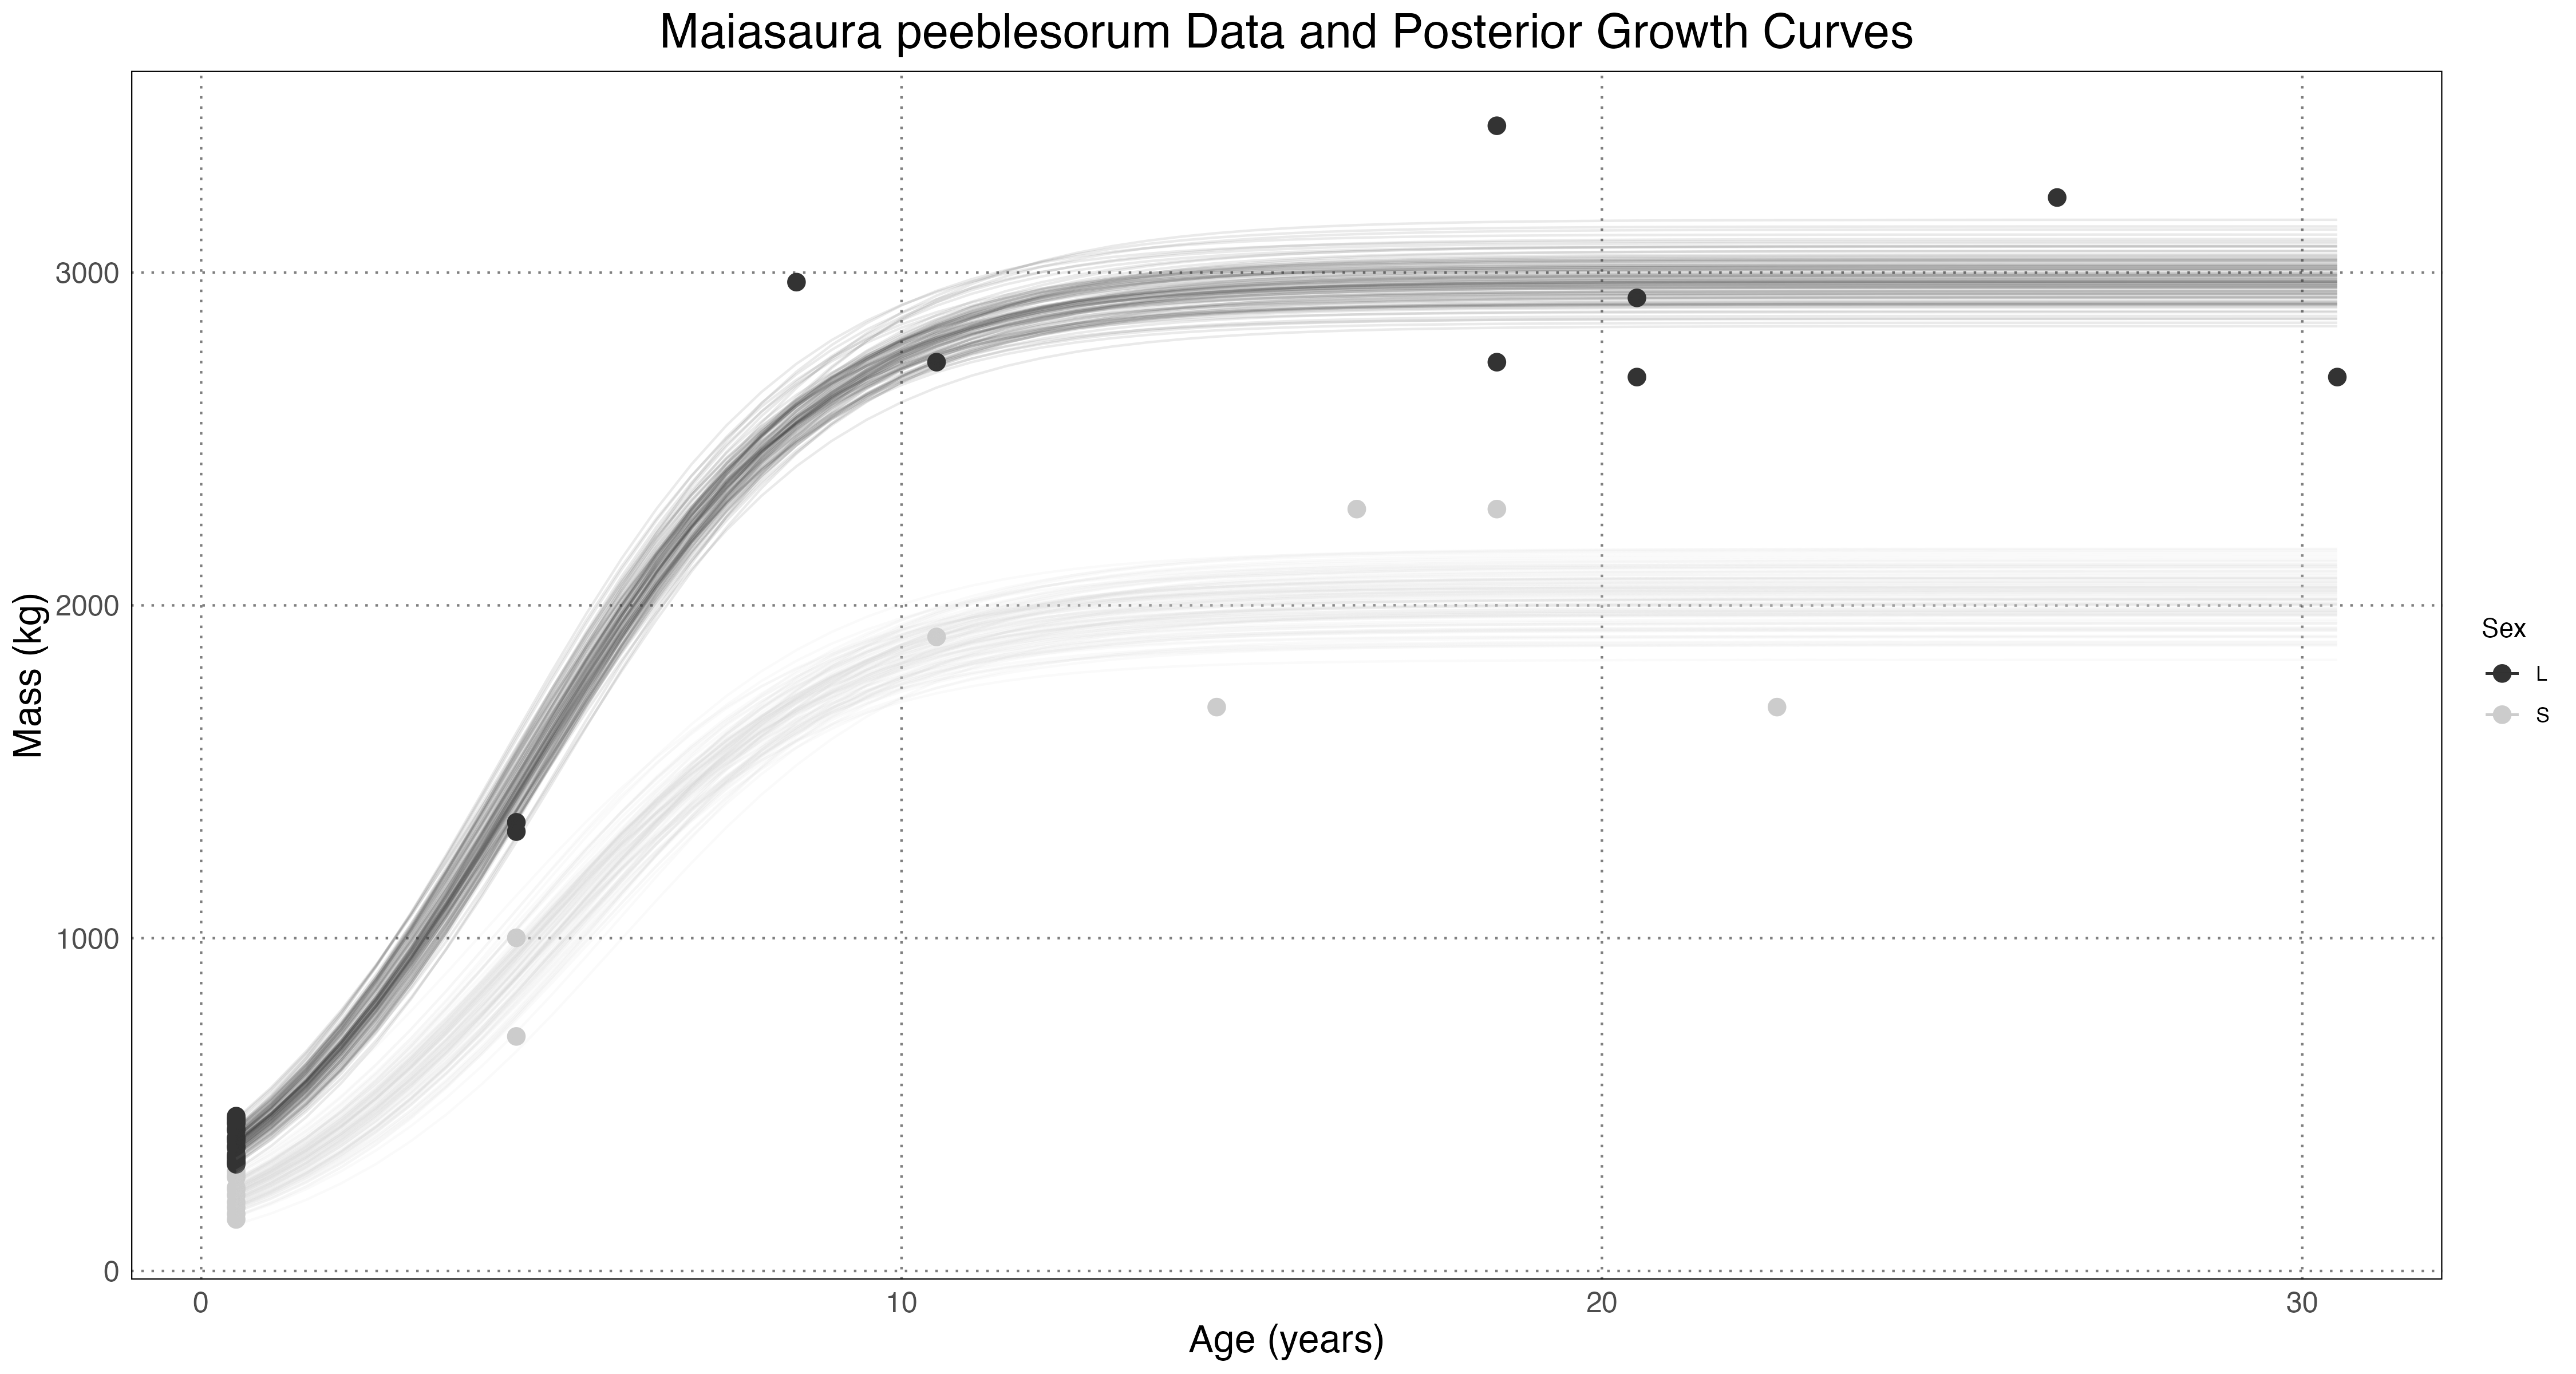
\includegraphics[width=\textwidth]{images/maiasauraPosterior.png}
  \end{minipage}
    \label{fig:maiasauraPriorPosterior}
    \caption{\maia{} Prior and Posterior Estimates}
\end{figure} 

\begin{figure}[H]
  \centering
  \begin{minipage}[b]{0.45\textwidth}
    \centering
    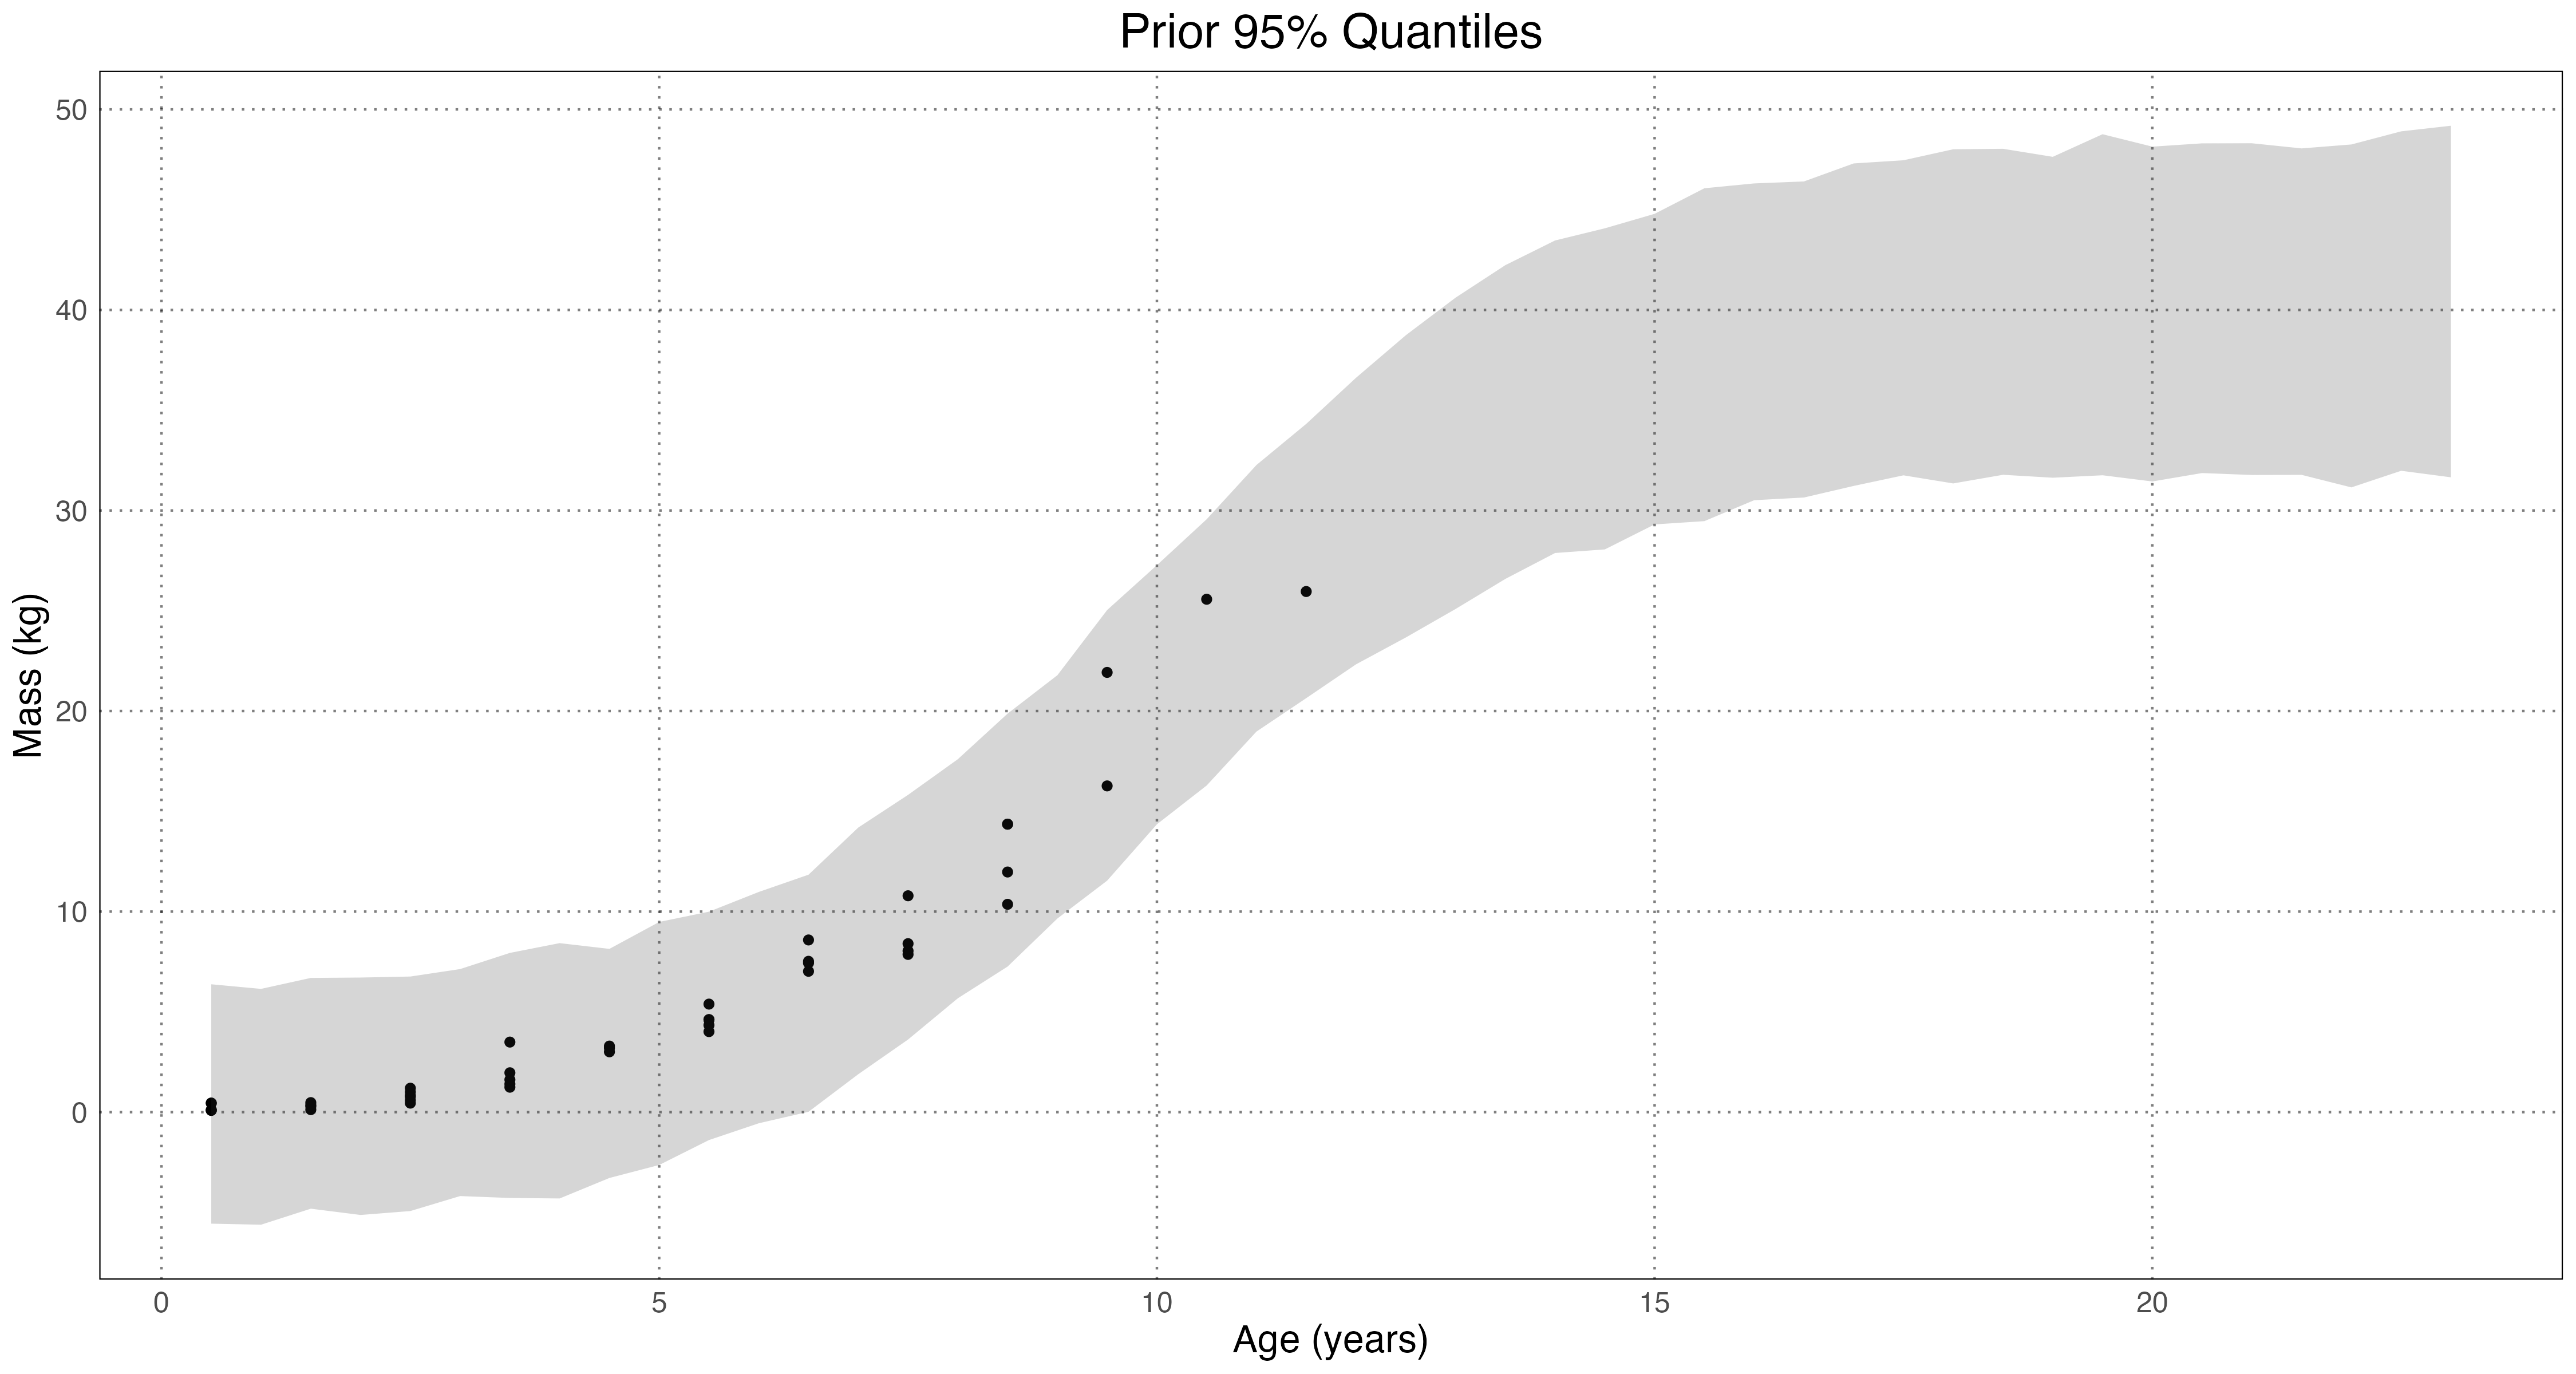
\includegraphics[width=\textwidth]{images/psittacosaurusPrior.png}
  \end{minipage}
  \begin{minipage}[b]{0.45\textwidth}
    \centering
    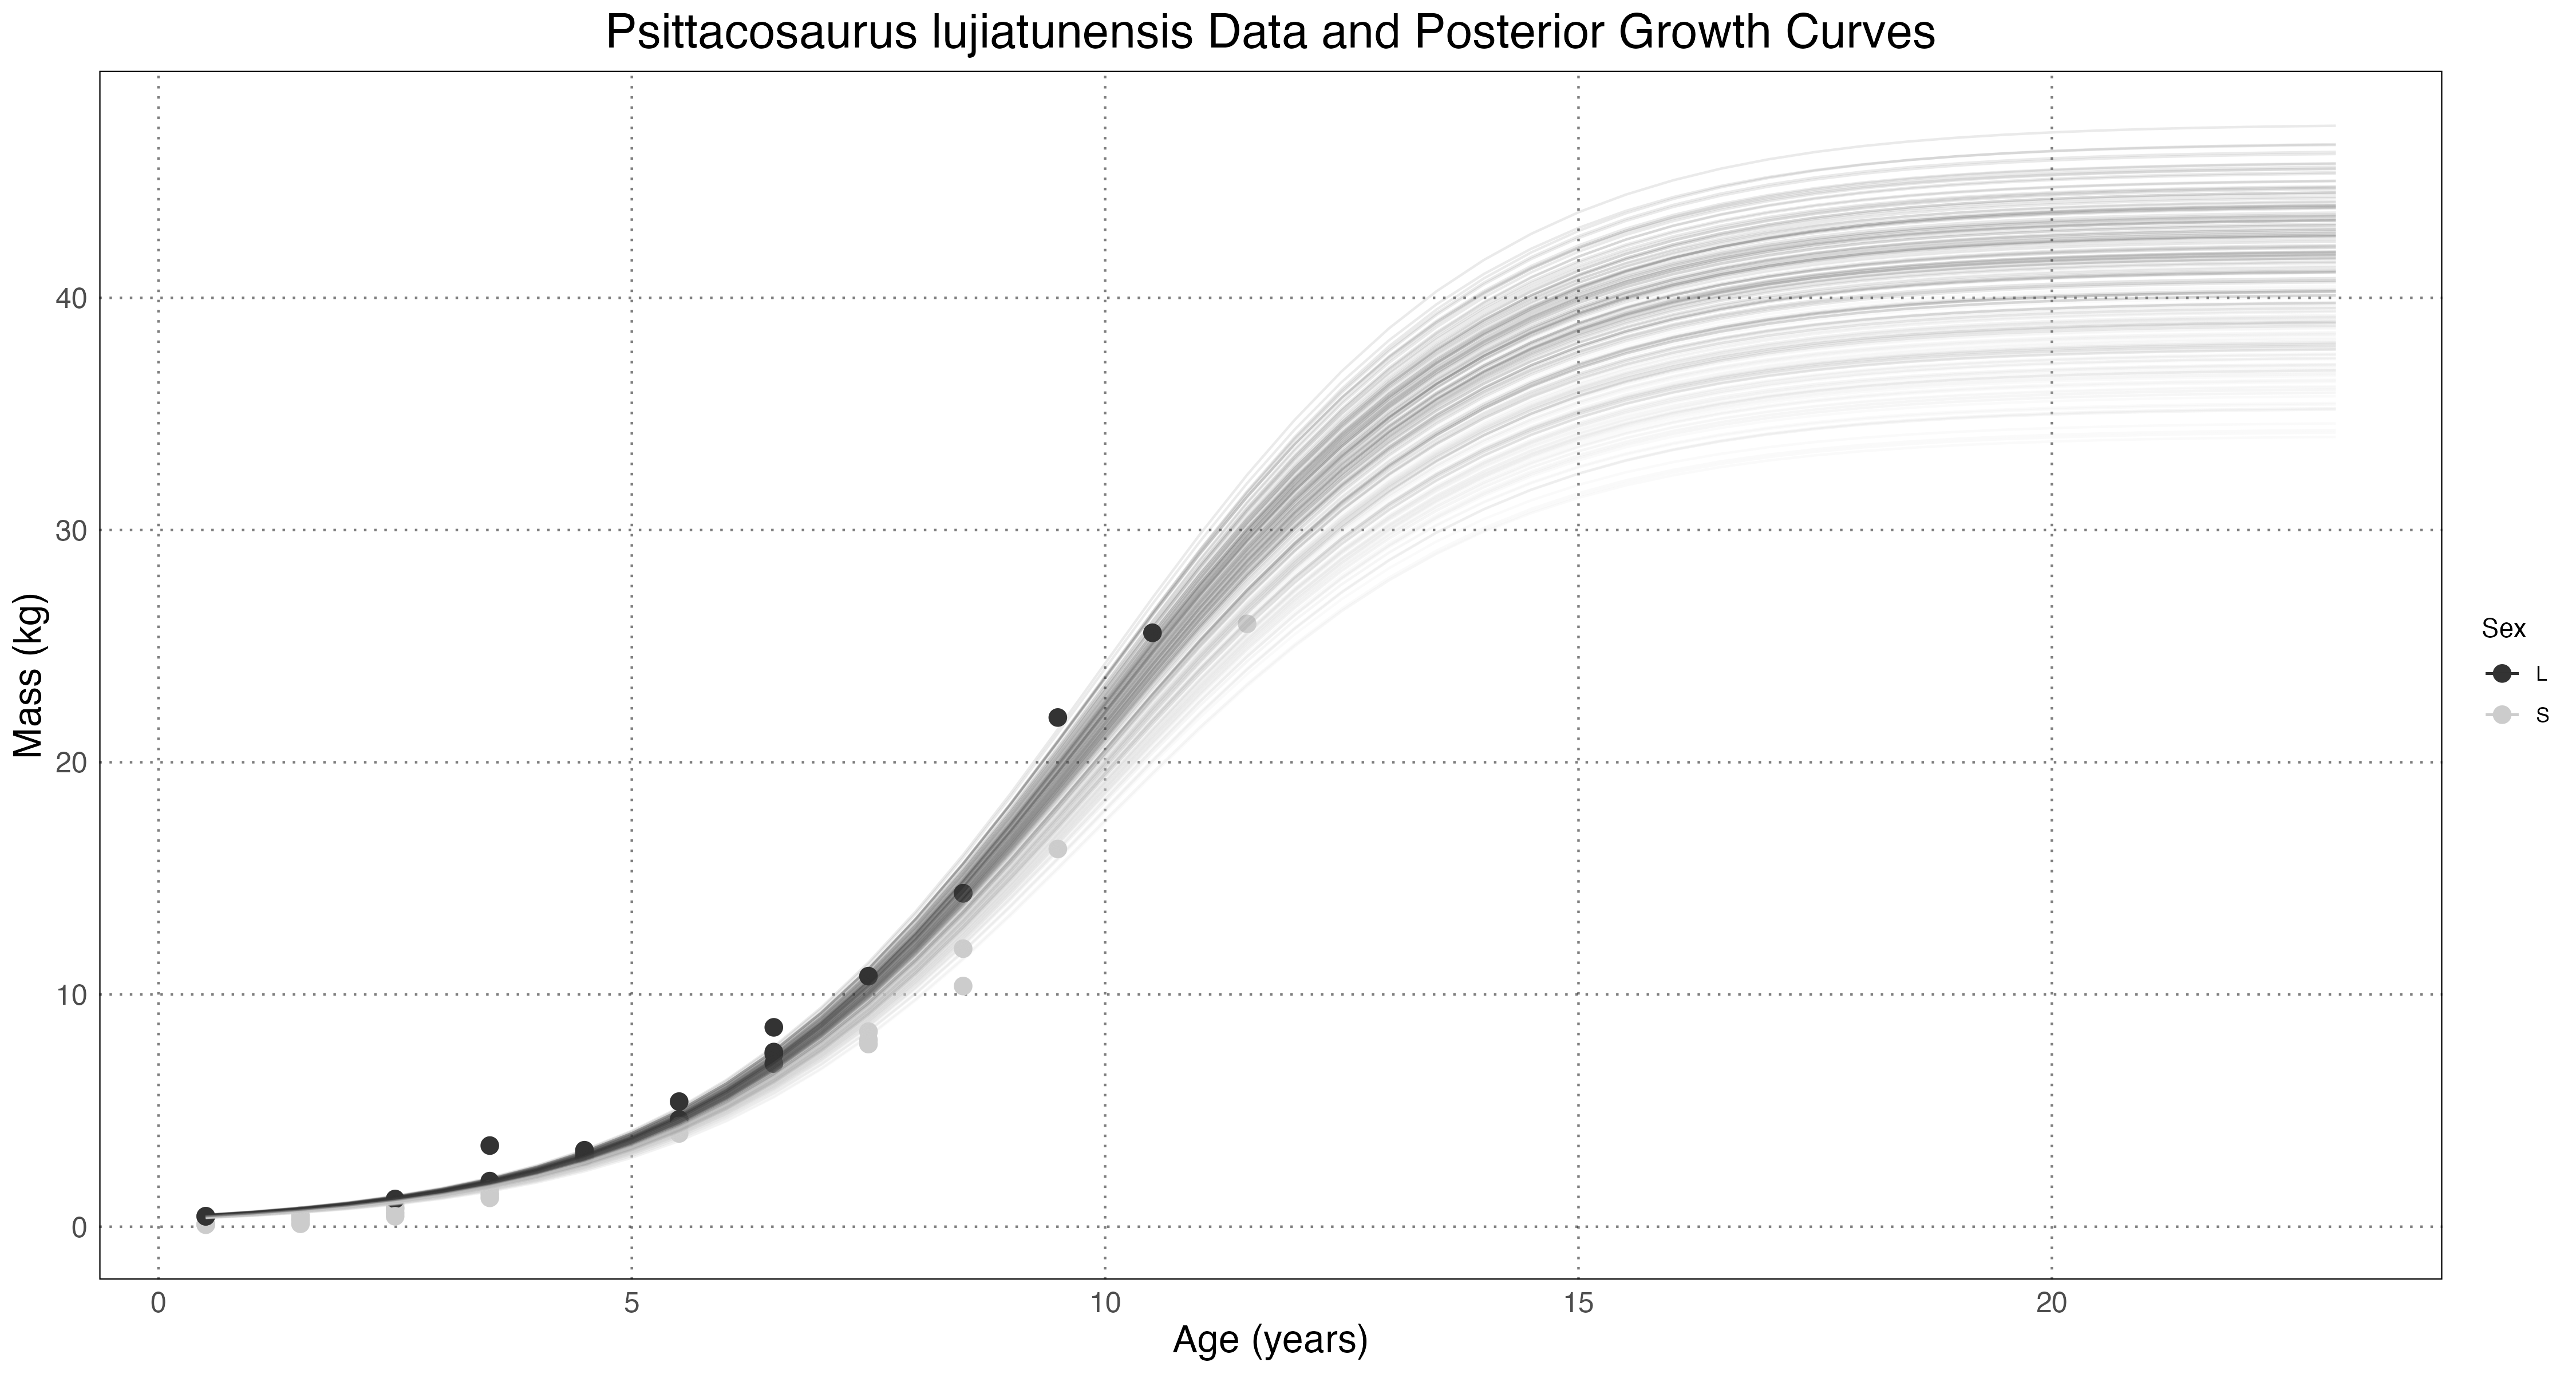
\includegraphics[width=\textwidth]{images/psittacosaurusPosterior.png}
  \end{minipage}
    \label{fig:psittacosaurusPriorPosterior}
    \caption{\psit{} Prior and Posterior Estimates}
\end{figure} 

\begin{figure}[H]
  \centering
  \begin{minipage}[b]{0.45\textwidth}
    \centering
    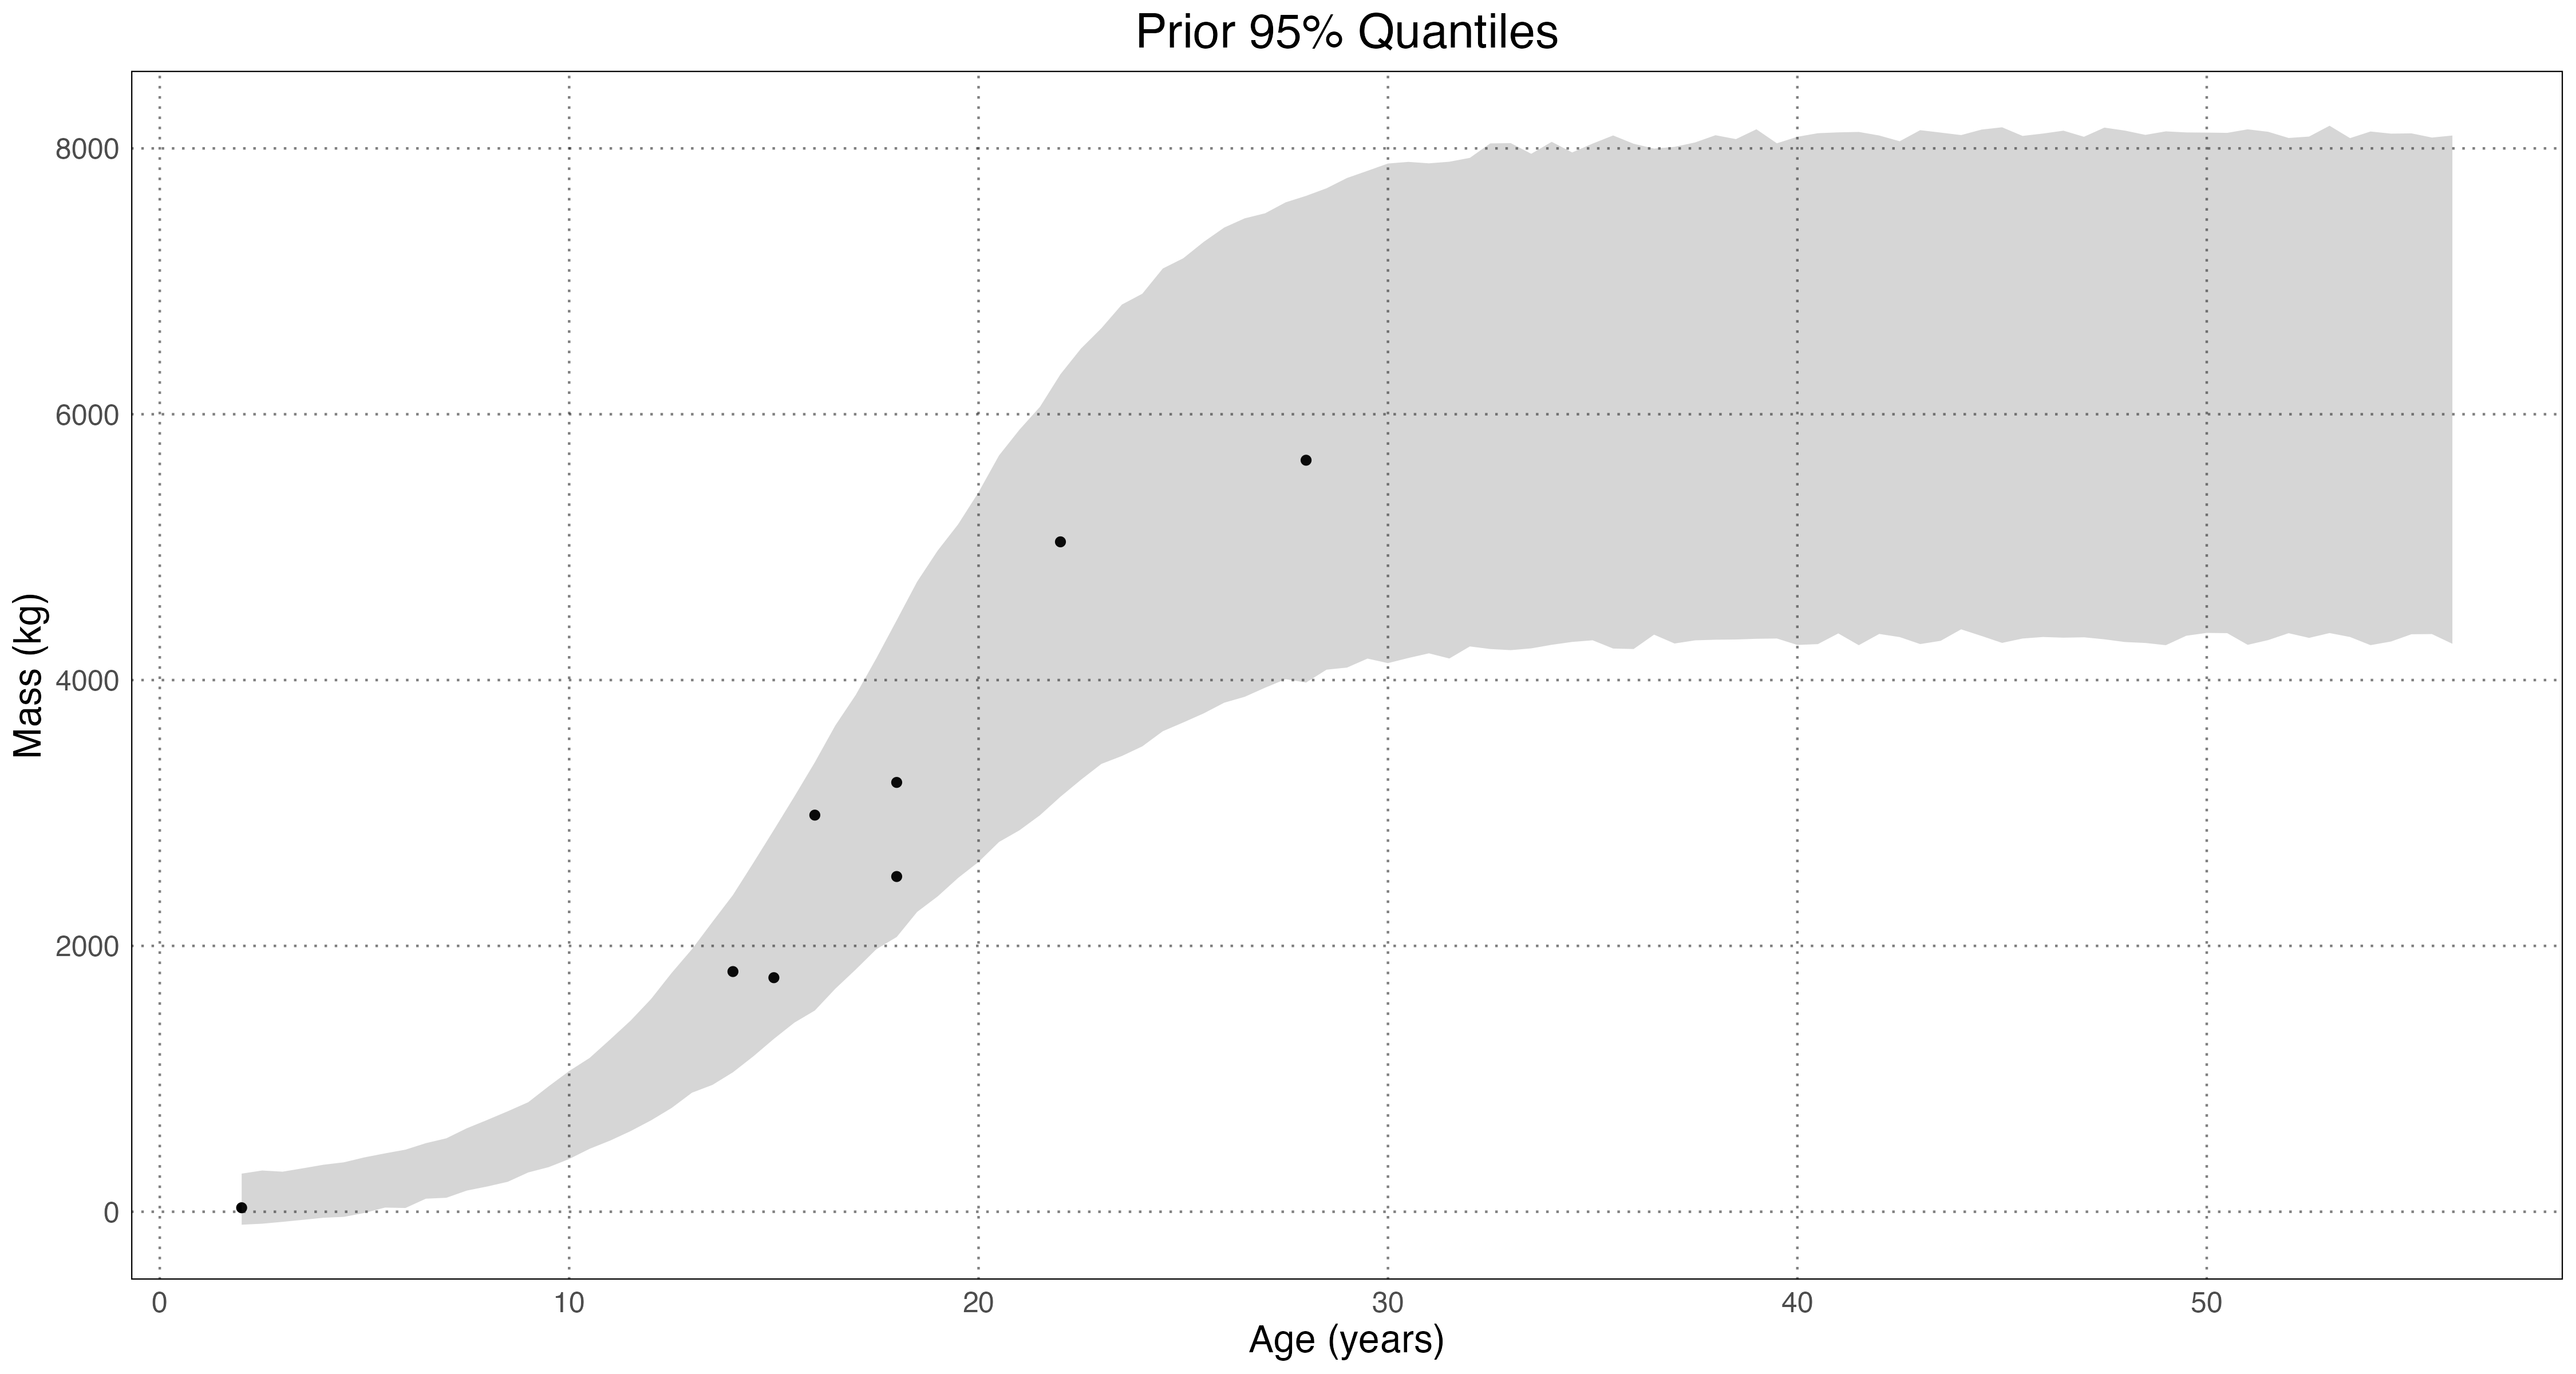
\includegraphics[width=\textwidth]{images/tyrannosaurPrior.png}
  \end{minipage}
  \begin{minipage}[b]{0.45\textwidth}
    \centering
    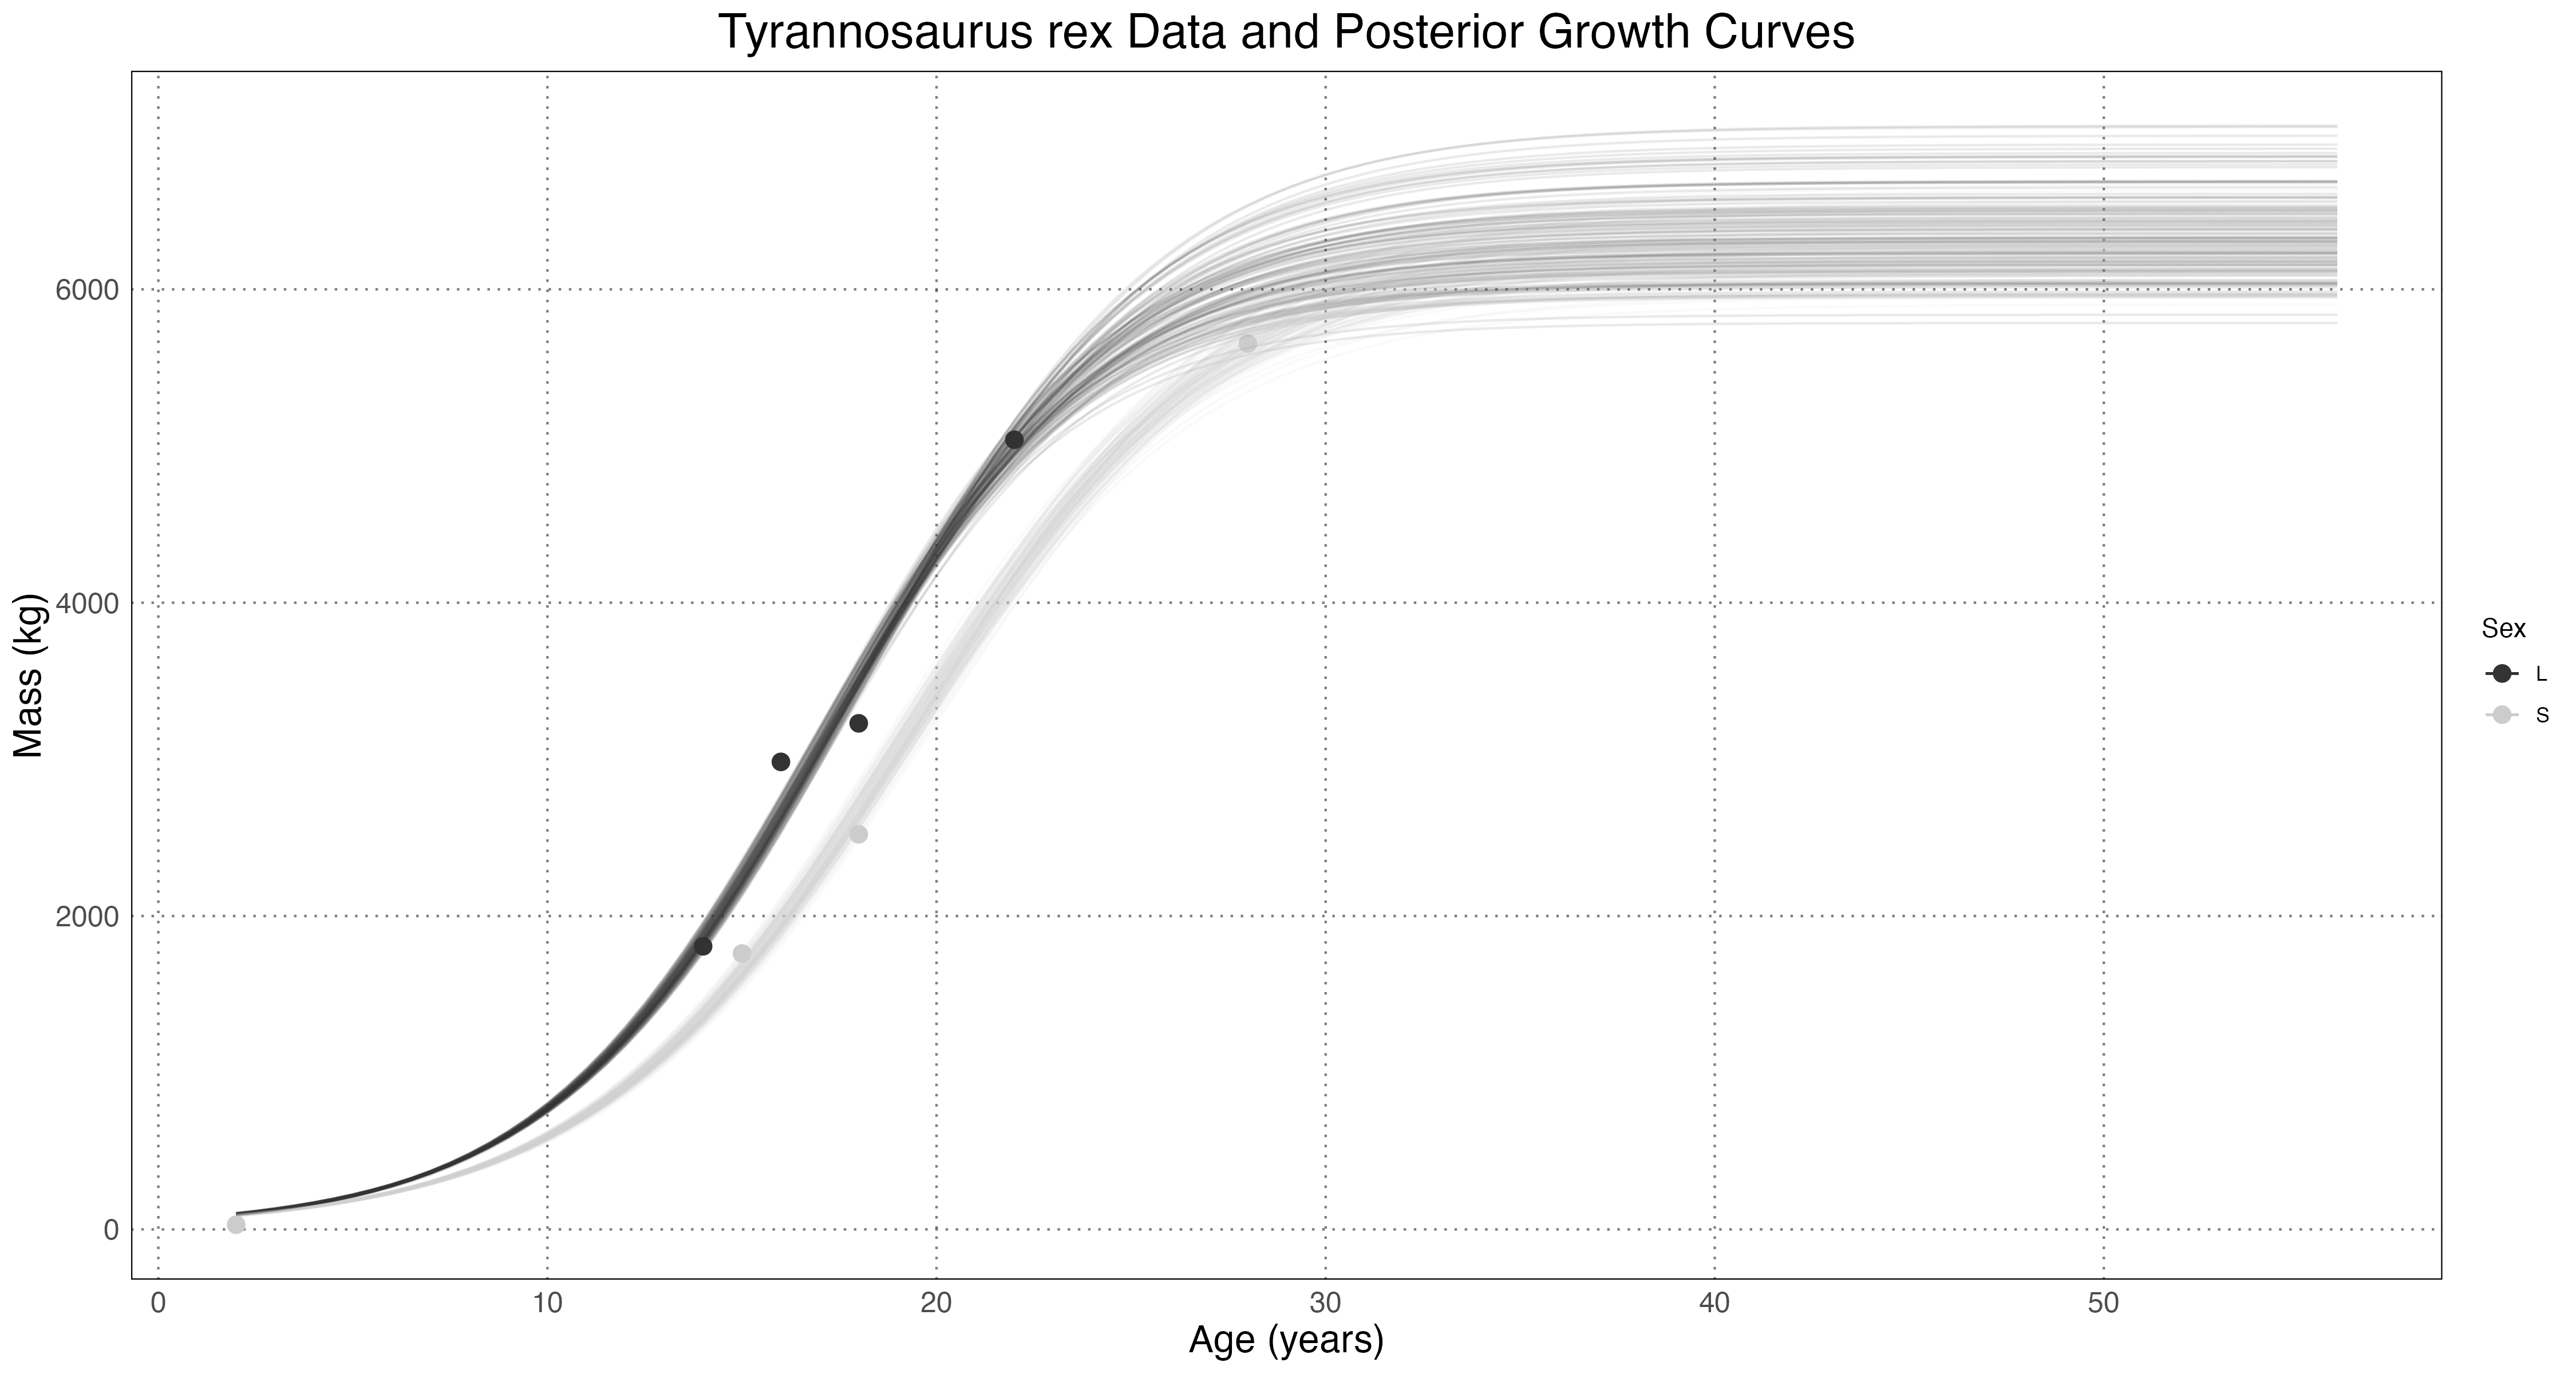
\includegraphics[width=\textwidth]{images/tyrannosaurPosterior.png}
  \end{minipage}
    \label{fig:tyrannosaurPriorPosterior}
    \caption{\tyran{} Prior and Posterior Estimates}
\end{figure} 

The posterior curves are biologically plausible and in line with both the data and our understanding of physiology; none of the values are immediately out of the realm of possibility.

Of course, we can also compare the levels of dimorphism as the larger sex's size as a percent of the smaller one (e.g. a dimorphism level of 50\% would mean that the larger sex was 50\% larger than the smaller).

\begin{figure}[H]
	\centering
	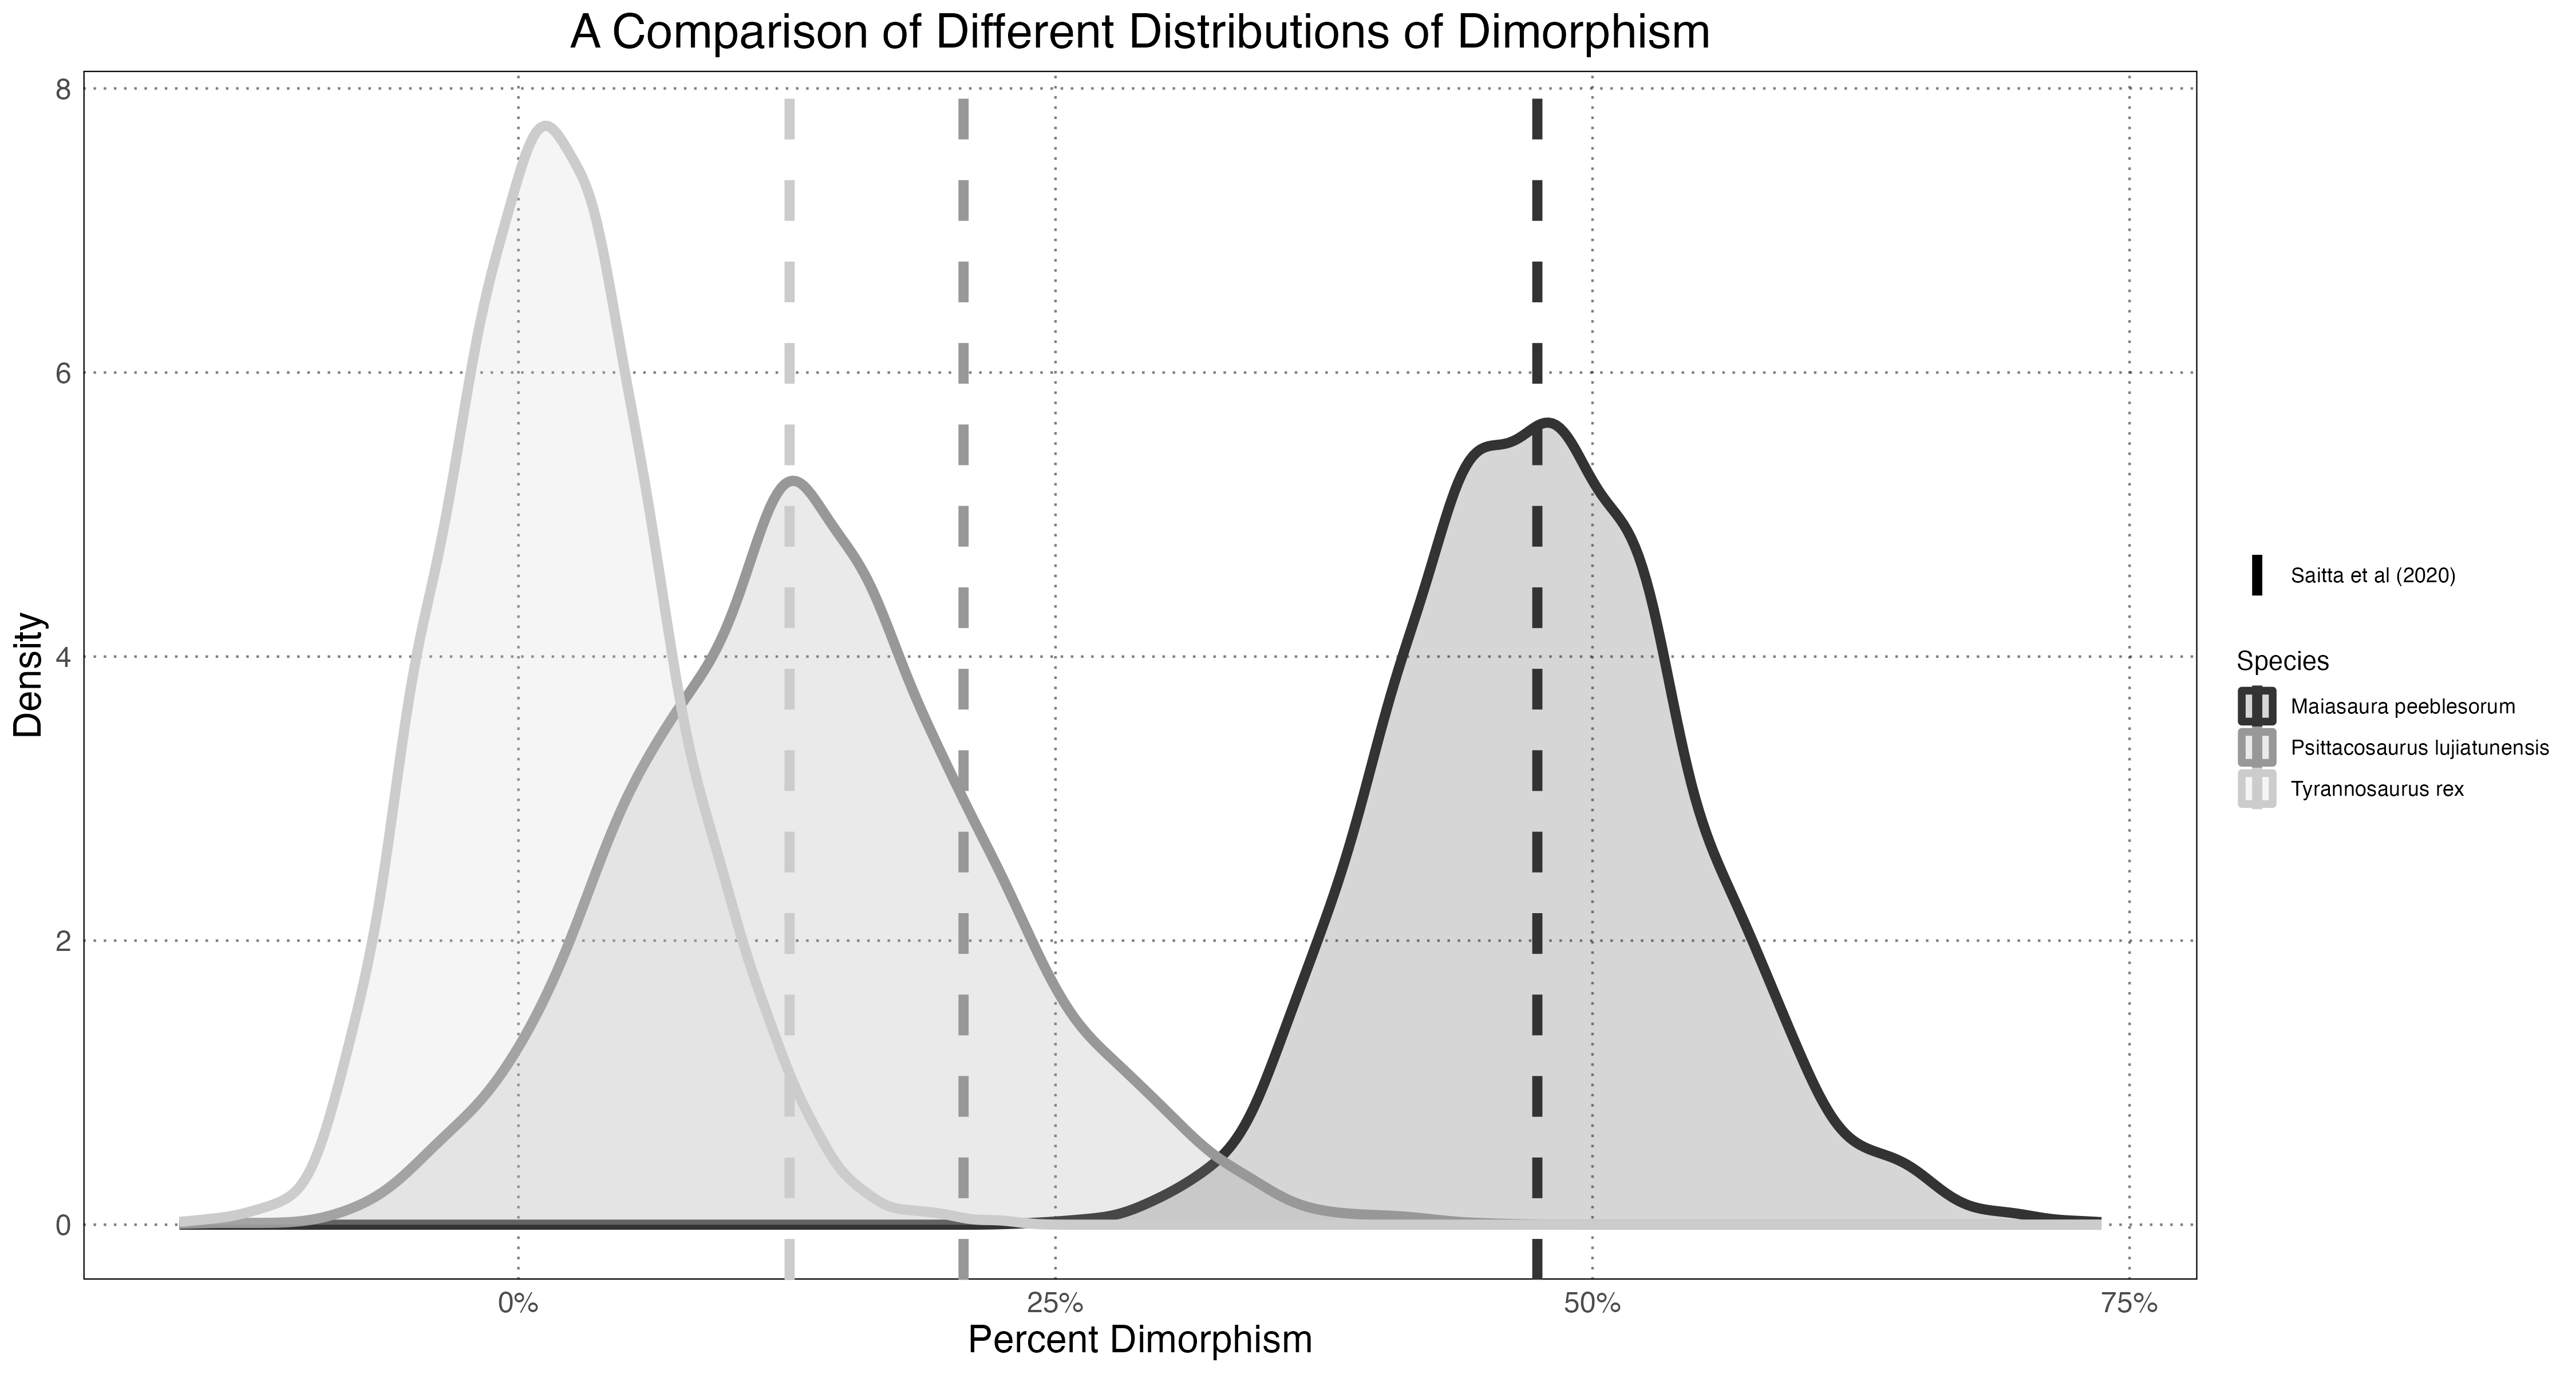
\includegraphics[width = 0.9\textwidth]{images/combinedDimorphism.png}
	\caption{Dimorphism Levels}
	\label{fig:combinedDimorphism}
\end{figure}

From this, we can see strong evidence for the \maia{} and \psit{} dimorphism, while the \tyran{} displays either no or a very small amount of dimorphism.

\section{Discussion}

As shown above, the modification of the method in \cite{saittaEffectSizeStatistical2020} using Bayesian regression to calculate the posterior distributions for sex-specific growth curves and the level of sexual dimorphism is generally reliable and useful way to quantify dimorphism in extinct populations. While it shares some weakness with with the original method, it also has several notable advantages. One is that by carrying uncertainty through all parts of modelling, the final result contains more information about the process \parencite{mcelreathStatisticalRethinkingBayesian2020}. Another is that by incorporating prior knowledge, we can constrain our final result to be biologically plausible.

Despite these advantages, there remain many area in which this method could be improved. The most critical, as noted in \cite{saittaEffectSizeStatistical2020}, is sex determination. As shown by Figure \ref{fig:alligatorSexPredictionError} sex determination accuracy was a strong predictor of the error in the level of dimorphism. There are two complementary paths which should be taken towards alleviating this issue. The first is the incorporation of the uncertainty in sex determination into the posterior curves generated. At the moment we behave as though the sex that we predict is correct, with no uncertainty, when the reality is that this is a significant source of error. This would result in widening the posterior distributions for the levels of dimorphism, but would not address the underlying issue. For that, we should look at alternate means of predicting sex, such as cluster analysis involving traits other than the one that we are looking at.

Determining levels of sexual dimorphism when both sex and size determination are difficult is naturally a difficult problem, and the method here, while offering an incremental improvement over existing methods, is certainly no panacea. Further efforts, both on the statistical and palaeontological side of the equation, will be required in order to improve our understanding of sexual dimorphism within extinct taxa.

\printbibliography[title=Bibliography]
\end{document}